\documentclass[10pt,final]{report}
\usepackage{fontspec}
\usepackage{libertine}
\usepackage{color}
\usepackage{graphicx}
\DeclareGraphicsExtensions{.png,.pdf,.jpg,.jpeg}
\usepackage{subcaption}
%%% The next two are necessary to get the degree symbol in text and math mode
\usepackage{textcomp}
\usepackage{gensymb}
\usepackage{hyperref}
\hypersetup{%
  colorlinks = true,
  linkcolor  = black,
  urlcolor   = cyan,
  plainpages = false,
  pdfencoding = auto
}
\usepackage{siunitx}
\sisetup{
	range-phrase = -,
	range-units = single,
	separate-uncertainty = true
}
% for chemical symbols, relevant for gas mixes, for example
\usepackage[version=4]{mhchem}
\usepackage{hepnames}
\usepackage[mathrm=sym, mathup=sym, mathit=sym, mathsf=sym, mathbf=sym, mathtt=sym]{unicode-math}
\defaultfontfeatures{Scale=MatchLowercase}
% \setmainfont{Linux Libertine O}
% \setsansfont{Linux Biolinum O}
% \setmathfont{TeX Gyre Termes Math}
% \setmonofont{Inconsolata}
\usepackage{pdfpages}
\usepackage{tabularx}
\usepackage{booktabs}
\usepackage{pdflscape}
\usepackage{multirow}
\usepackage[export]{adjustbox}
\usepackage{geometry}
\usepackage[backend=biber,sorting=none]{biblatex}
\usepackage{xspace}
\usepackage{enumitem}

\addbibresource{detectorRnD.bib}
\DeclareBibliographyDriver{caliceanalysisnote}{%
    \printnames{author}%
    \newunit\newblock
    \printfield{title}%
    \newunit\newblock
    \printfield{url}%
    \finentry%
}

\DeclareBibliographyDriver{eudetmemo}{%
    \printnames{author}%
    \newunit\newblock
    \printfield{title}%
    \newunit\newblock
    \printfield{url}%
    \finentry%
}

\DeclareBibliographyDriver{eudetreport}{%
    \printnames{author}%
    \newunit\newblock
    \printfield{title}%
    \newunit\newblock
    \printfield{url}%
    \finentry%
}

\DeclareBibliographyDriver{presentation}{%
    \printnames{author}%
    \newunit\newblock
    \printfield{title}%
    \newunit\newblock
    \printfield{conference}%
    \newunit\newblock
    \printfield{location}%
    \newunit\newblock
    \printfield{year}%
    \newunit\newblock
    \printfield{url}%
    \finentry%
}

\newcommand{\LYCORIS}{{\textsc{Lycoris}}\xspace}
\newcommand{\DESYII}{{\mbox{DESY II}}\xspace}
\newcommand{\DIITBF}{{\DESYII Test Beam Facility}\xspace}
\newcommand{\SID}{{SiD}\xspace}
\newcommand{\KPIX}{{KPiX}\xspace}

\begin{document}


\begin{titlepage} 
    \newcommand{\HRule}{\rule{\linewidth}{0.5mm}} % Defines a new command for horizontal lines, change thickness here
	\center % Centre everything on the page
	
	%------------------------------------------------
	%	Headings
	%------------------------------------------------
	
	\textsc{\LARGE Linear Collider Collaboration}\\[1.5cm] % Main heading such as the name of your university/college
		
%	\textsc{\large Minor Heading}\\[0.5cm] % Minor heading such as course title
	
	%------------------------------------------------
	%	Title
	%------------------------------------------------
	
	\HRule\\[0.4cm]
	
	{\huge\bfseries Detector R\&D Report}\\[0.4cm] % Title of your document
	
	\HRule\\[1.5cm]

	% FIXME For the final version, make the version number large again and remove "Draft" and the deadline
    \textsc{\Large Final Version}\\[0.5cm] % Major heading such as course name
	\href{https://doi.org/10.5281/zenodo.3749461}{doi:10.5281/zenodo.3749461}\\[1cm]
	%------------------------------------------------
	%	Editors
	%------------------------------------------------
	\vfill\vfill
	{\large Editors\\}
	\begin{minipage}[t]{0.49\textwidth}
		\begin{flushleft}
			\large
			\textit{Detector R\&D Liaison}\\
			Maxim \textsc{Titov} \\
			Institut de Recherche sur les lois Fondamentales de l'Univers (IRFU) \\
			CEA - Saclay, F-91191 Gif-sur-Yvette Cedex, France\\
			maxim.titov@cea.fr
		\end{flushleft}
	\end{minipage}\hfill
	\begin{minipage}[t]{0.49\textwidth}
		\begin{flushright}
			\large
			\textit{Detector R\&D Liaison}\\
			Jan F \textsc{Strube} \\
			Pacific Northwest National Laboratory \\
			902 Battelle Boulevard \\
			Richland, WA 99352, USA \\
		\end{flushright}
			\begin{flushright}
				\large
			University of Oregon \\
			Institute for Fundamental Science \\
			Eugene, OR 97403, USA \\
			jstrube@uoregon.edu
			\end{flushright}
	\end{minipage}
		
	%------------------------------------------------
	%	Date
	%------------------------------------------------
	\vfill\vfill\vfill % Position the date 3/4 down the remaining page
	{\large\today} % Date, change the \today to a set date if you want to be precise
	
	%------------------------------------------------
	%	Logo
	%------------------------------------------------
	
	\vfill\vfill
    \includegraphics[width=0.4\textwidth]{signature_red2-cmyk}\\[1cm] % Include a department/university logo
    %\includegraphics[width=0.15\textwidth]{logo_red2-cmyk}\\[1cm] % Include a department/university logo 
    %\includegraphics[width=0.2\textwidth]{logotype_red2-cmyk}\\[1cm] % Include a department/university logo 	 
	%----------------------------------------------------------------------------------------
	
	\vfill % Push the date up 1/4 of the remaining page
	
\end{titlepage}

\tableofcontents
\chapter*{Foreword}
\section*{Linear Collider Detector R\&D Liaison Charge, as defined by the Linear Collider
Collaboration (LCC) Physics and Detector Executive Board Mandate (2014-2020):}
The LC Detector R\&D Liaisons ensure productive communication between the Linear
Collider Collaboration (LCC) Physics and Detectors Executive Board and the detector R\&D
groups. The liaisons are in contact with all individual detector R\&D groups relevant to linear
colliders to keep track of the overall detector R\&D activities conducted or planned for linear
colliders and to periodically compile summaries of the efforts. The report is not intended to
serve as the summary to select between different technologies or advertise the most
advanced ones, but rather as the general overview of the Linear Colliders Detector R\&D
landscape.


\section*{Introduction}
The physics goals of high-luminosity particle accelerators, from LHC to the High-
Luminosity LHC (HL-LHC) and to the
next generation of lepton colliders, have set quite stringent constraints on the future needs at
the Instrumentation Frontier. Many technologies are reaching their sensitivity limit and new
approaches need to be developed to overcome the currently irreducible technological
challenges. The detrimental effects of material budget and power consumption present
a very serious concern for high-precision silicon vertex and tracking detectors. One of the
most promising areas is CMOS sensors, which offer low mass and potentially radiation-hard
technology for future proton--proton and electron--positron colliders, intensity frontier and
heavy-ion experiments. MPGDs have become a well-established technology in the fertile field
of gaseous detectors; these will remain the primary choice, whenever large-area
coverage with low material budget is required. Vacuum tube technology is inherently fast and
new developments include advances in micro-channel plates for photomultipliers with a
potential for picosecond-time resolution in large systems. Several novel concepts of
picosecond-timing detectors will have numerous powerful applications in particle
identification, pile-up rejection and event reconstruction, and serve numerous scientific goals.
The story of modern calorimetry is a textbook example of physics research driving the
development of an experimental method. Silicon photomultipliers have seen a rapid progress
in the last decade, becoming the standard solution for scintillator-based devices. The
integration of advanced electronics and data transmission functionalities plays an
increasingly important role and needs to be addressed. Future experimental projects also
face a large number of diverse engineering challenges, in the areas of system integration,
power distribution, cooling, mechanical support structures, and production techniques.
Bringing the modern algorithmic advances from the field of machine learning from offline
applications to online operations and trigger systems is another major challenge. The
timescales spanned by future projects in particle physics, ranging from few years to many
decades, constitute a challenge in itself, in addition to the complexity and diversity of the
required accelerator and detector R\&D.

The landscape of proposed future accelerator facilities is broad in terms of detector
technologies to address the physics programs. At the Energy Frontier one can distinguish
two major drivers for detector R\&D in the short term: detector upgrades toward HL-LHC
and development of advanced technologies for future $\mathrm{e}^{+}\mathrm{e}^{-}$
linear colliders (ILC, CLIC). The latter are inherently very accurate physics probes requiring
integrated concepts with ultimate precision, minimal power consumption and ultra-light
structures. A key challenge to demonstrate the required detector performance in a realistic
environment represents a major step forward toward a complete system. Fast and accurate
physics-driven detector simulations have gained considerable importance with the increase of
the complexity of novel instrumentation. Concerning synergies and challenges in the design
and instrumentation developments for the ILC and CLIC (and future circular lepton collider)
experiments, these are in most cases orthogonal to the main directions of HL-LHC
experiments. Rather than emphasizing radiation hardness and rate capability, the demands
for resolution (granularity) and material budget on one hand, and for acceptable speed and
low power consumption on the other hand, exceed significantly what is the state-of-the-art today.
Such leaps in performance cannot be achieved by simple extrapolation of the known, but
only by entering new technological territory in detector R\&D. Several new concepts for silicon
sensor integration, such as monolithic devices, are being pursued for pixel vertex detectors,
new micro-pattern gas amplification techniques are under study for tracking and muon systems,
and the particle-flow approach to calorimetry promises to deliver unprecedented jet energy
resolution, to name just some examples.

Emerging novel detector technologies are the vital backbone for the success of the
upcoming large and complex particle physics experiments. They are usually the result of a
long development cycle encompassing many stages: generic ``blue-sky'' R\&D and R\&D
activities guided by the needs of future projects, focused R\&D activities for an approved
experiment, production, industrialization and installation/commissioning, where engineering
aspects play a very important role. On average, it might take more than 20 years to mature a
technology from the original idea to a well-established technique suited for implementation
(e.g.\ the first workshop on the LHC was held in 1984).

Over the past few decades, a large number of groups have pursued extensive generic
detector R\&D studies, summarized in this report, applicable to any of the proposed Linear
Collider detector concepts (International Large Detector (ILD), Silicon Detector (SiD) and
CLIC Detector and Physics (CLICdp). Intentionally, these groups did not yet make very
specific choices and keep various options for technologies to realise the individual sub-
detectors. This has the advantage that the technologies can be further developed until
specific choices have to made, once the project is approved. Furthermore---and as important---this
keeps a broad community of detector research groups at universities and laboratories
involved and increases the chance to arrive at the best technically possible detector solution
when it has to be built. Wherever possible, the R\&D is not pursued with respect to one
specific concept but in the context of world-wide transversal R\&D collaborations which work
on technologies rather than detector designs, such as CALICE, LCTPC, and FCAL. Further
R\&D programs are ongoing, e.g.\ for various monolithic pixel detector technologies
(CMOS, DEPFET, FPCCD, SoI), for generic aspects of the next generation silicon vertex
detectors for Linear Colliders and for the development of forward calorimetry. Last, but not
least, European Commission-funded programs, such as EUDET, AIDA/AIDA2020 and
ATTRACT play an important role in enabling and supporting generic R\&D activities.
This report provides an overview of the past and presently ongoing Linear Collider
detector R\&D studies, including those not directly included in the ILD, SiD and CLICdp
concept groups today, but which might become relevant in the future. The main purpose of
the document is to summarize recent progress, followed by the description of future
milestones, with the following goals:
\begin{itemize}
	\item ``Publicize'' particular technology and to provide an update of the recent R\&D efforts
since the Conceptual Design Report (CDR) for CLIC and the Detailed Baseline
Design (DBD) for the ILC;
	\item Provide a ``snapshot'' for a given technology, without information on manpower needs
and financial resources to reach project milestones. As most detector R\&D groups
are highly independent with their own funds, this document is not intended to serve
as a guideline to control or coordinate different R\&D efforts, by indicating potential
overlap areas;
	\item Provide an entry point for new groups in order to help them learn about the current
landscape of LC R\&D efforts and the areas where they might be interested to
contribute.
\end{itemize}
Therefore, each individual R\&D group within the Linear Collider community was asked to
submit a short document answering five questions in relation to their R\&D program, as an
input to the Linear Collider Detector R\&D Liaison report. These are:
\begin{itemize}
	\item Introduction. Brief overview of the technology (past R\&D efforts with references);
	\item Recent milestones since ILC DBD and CLIC CDR publications;
	\item Engineering challenges for a given detector technology in order to encourage new
groups to contribute to the engineering aspects and not only to the generic R\&D;
	\item Future plans in the years to come and the list of collaborating institutes;
	\item R\&D spin-offs beyond the ILC, if technology has been already used in other projects.
\end{itemize}
The LC Detector R\&D Liaison report served as an online documentation, updated on a
regular basis and available to community and newcomers, during the LCC Physics and
Detector Executive Board mandate (2014-2020).

In particular, version 2018.3 (released December 17, 2018) was used as one of the main
LCC supporting documents presented to the European Strategy Process:
\url{https://ilchome.web.cern.ch/content/ilc-european-strategy-document.html}
This version represents the final release of the Linear Collider Detector R\&D report at the
end of the LCC mandate. It is intended to serve as one of the inputs to the US Snowmass
process: \url{https://snowmass21.org/}.

\chapter{Vertex Detectors}
\input{VertexDetector/Motivation}
\section{CMOS}
Most recent update: 2020-04-25 \\
Contact person: Marc Winter (email: marc.winter@iphc.cnrs.fr)

\subsection{Introduction}
CMOS Pixel Sensors (CPS) combine high granularity with low material
budget and allow integrating the full signal processing circuitry on
the sensor substrate. They benefit from a steady technological progress 
driven by an industrial market which makes them simultaneously cost 
effective and attractive for a wide range of applications. They are 
developed for an ILC vertex detector since about two decades and were 
shown to rather easily comply with the required spatial resolution 
and material budget expressed in the DBD~\cite{Behnke:2013lya}. The
associated read-out time of a few tens of microseconds represented the
limit achievable with a rolling shutter read-out and the \SI{350}{\nano\meter} CMOS 
technology available at that time. The required radiation tolerance, 
on the other hand, was observed to be well within the sensor potential.
 
The relevance of the technology for subatomic physics experiments is established today with the 400 ULTIMATE sensors operated in the STAR-PXL 
detector~\cite{CONTIN201860} at RHIC/BNL from 2014 to 2016, while the
state of the art is well illustrated by the $\sim$ 20 times faster ALPIDE sensors fabricated ($>$ 20,000 dies) in a \SI{180}{\nano\meter} CMOS technology, to 
equip the upgraded, $>$ \SI{10}{\meter\squared} large, ALICE Inner Tracker System 
(ITS)~\cite{AGLIERIRINELLA2017583}. 
The variety of devices where ULTIMATE has been implemented and, even 
more so, where ALPIDE is foreseen to be integrated, reflects the maturity 
of the technology and the steadily growing interest it generates in the
field.
 
  The detection performances achieved at the time of the DBD 
assumed that integrating the beam related background over several tens 
of bunch-crossings would result in a well affordable disturbance of the 
event reconstruction. Since then, 
potential benefits from shorter integration times, allowing for bunch 
tagging or nearly so, have become clearer and desirable. This applies 
for instance to the distinction between soft tracks due to beamstrahlung
or two-photon collisions and those originating from a displaced vertex
and therefore contributing to the vertex charge. The latter may get  
particularly complicated to reconstruct in case of a higher machine 
luminosity than foreseen in the TDR and of worse running conditions 
than anticipated. 
  
  However, the goal of suppressing the impact of beam related background 
on the physics performance by improving the sensor time resolution to 
$\lesssim$ \SI{1}{\micro\second} steps up the preexisting tension between the 
small pixel size imposed by the required spatial resolution and the 
minimal space needed to implement the very front end circuitry inside 
the pixels. The R\&D pursued so far did not show that a spatial 
resolution of $\lesssim$ \SI{3}{\micro\meter} and a single bunch tagging are 
actually achievable simultaneously within the same, \SI{50}{\micro\meter} thin, 
sensor with the presently available CMOS technologies, moreover with 
a power consumption compatible with air cooling. On the other hand, 
$\sim$ \SI{4}{\micro\meter} spatial resolution may be within reach with sensors 
featuring a continuous read-out time of $\lesssim$ \SI{1}{\micro\second} at an 
affordable power consumption.

  Indirect approaches are therefore being considered to achieve the 
targeted spatial and time resolutions per layer even if they cannot be
reached within a single sensor. They rely on the concept of double-sided detector layers, which provides two hits, one per layer face, for each traversing charged particle. The track 
position and timing are extracted from the combination of the two 
signals delivered by sensors facing each other in the same layer. 
The position and timing may, for instance, come from a high precision 
sensor located on one layer side and a faster, less precise, sensor 
located on the opposite side. Alternatively, the spatial resolution 
may be derived from the combination of opposite, identical, sensors 
limited to \SI{4}{\micro\meter} spatial resolution measurements but providing 
both $\lesssim$ \SI{1}{\micro\second} read-out time.     

\begin{figure}
	\centering
	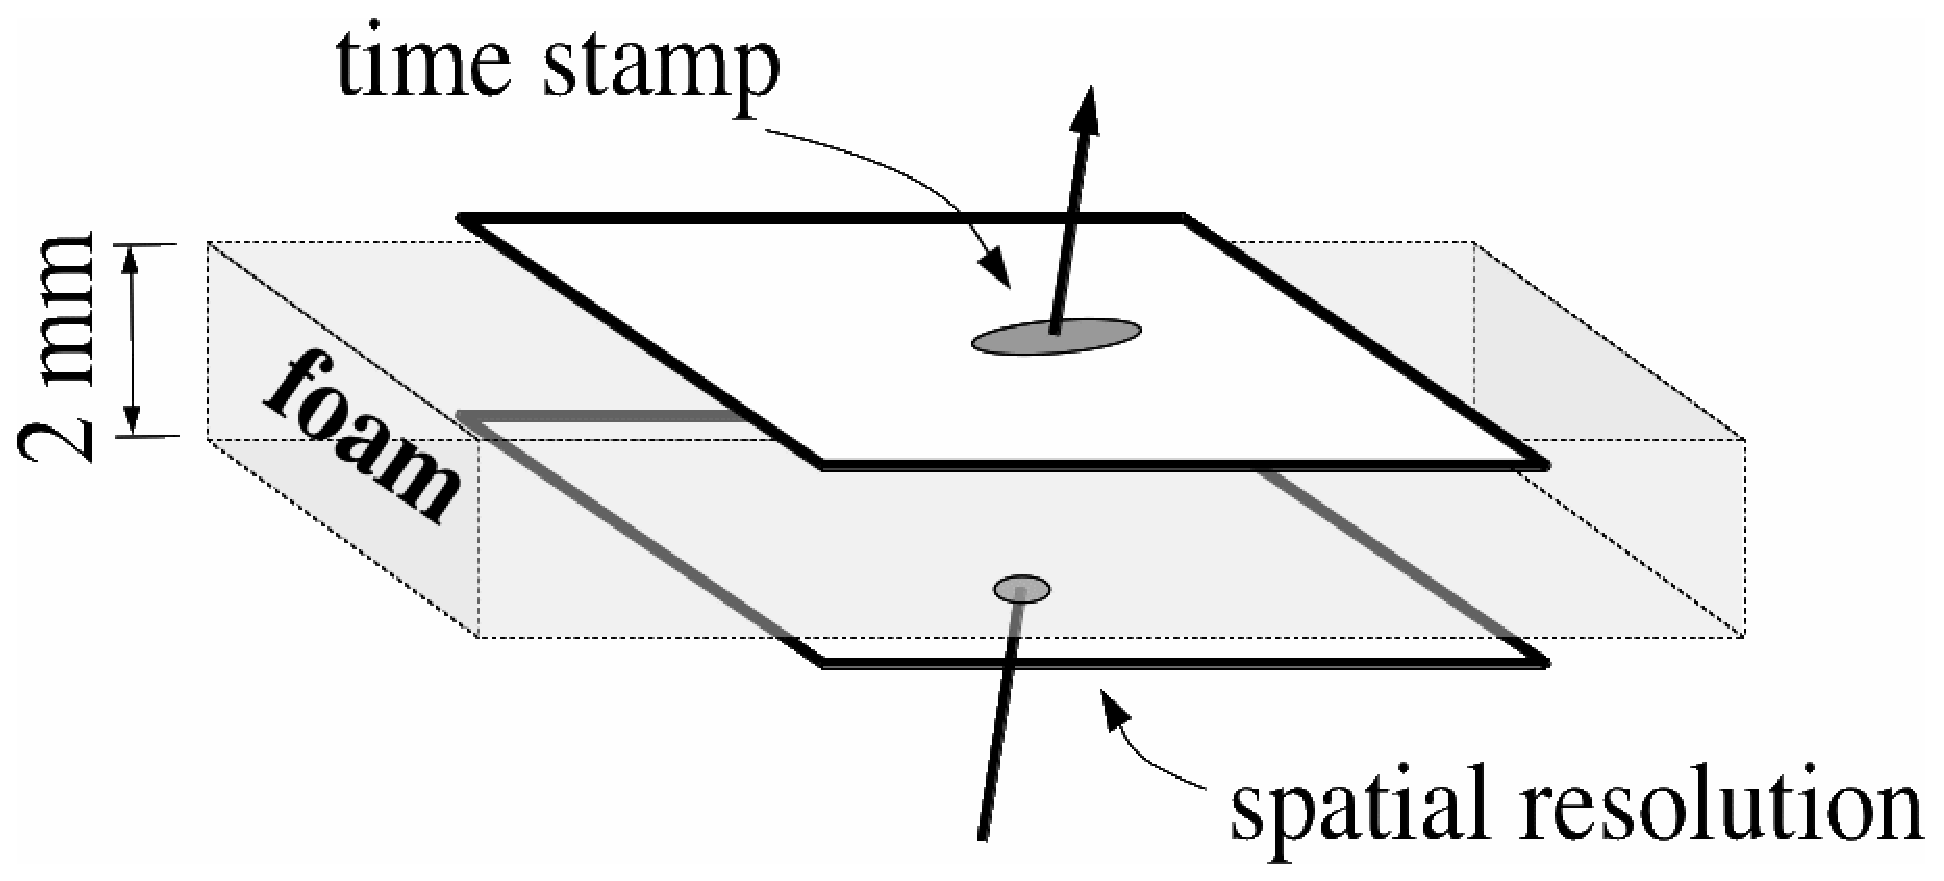
\includegraphics[width=.43\linewidth]{VertexDetector/CMOS/principe-MixedLayers-noPixels.eps}
	\includegraphics[width=.55\linewidth]{VertexDetector/CMOS/principe-MixedLayers-intermediatePoint.pdf}
	\caption{Alternative approaches based on double-sided layers. Left: particles traverse a "pointing" sensor and a ``timing'' sensor equipping the two faces of a layer. Right: the signals of two ``timing'' sensors featuring $\sim$ \SI{4}{\micro\meter} resolution are combined into a single signal to obtain the required spatial resolution of $\lesssim$ \SI{3}{\micro\meter}.}
	\label{fig:VertexDetector:CMOS:minivectors}
\end{figure}

\subsection{Recent Milestones}
The most advanced CPS under development extendable to bridge the 
gap between ALPIDE and a sensor adapted to an ILC vertex detector 
is the MIMOSIS sensor~\cite{Morel:mimosis}, which is foreseen to 
equip the 4 double-sided stations of the MicroVertex Detector (MVD) 
of the CBM heavy ion experiment at FAIR/GSI. The sensor acts 
simultaneously as a forerunner of a sensor suited to an ILC vertex 
detector. With a pixel array continuous read-out derived from ALPIDE, 
MIMOSIS features a 50 times higher hit density treatment capability 
and a \SI{5}{\micro\second} read-out time. The latter may be compressed to 
$\sim$ \SI{2}{\micro\second} for an ILC vertex detector, with an instantaneous 
power density in the order of $\sim$ SI{50 -- 150}{\mili\watt\per\centimeter\squared}, depending 
on the beam background induced hit density, and thereby on the 
distance to the interaction point. Such performances should allow 
facing the most pessimistic predictions for the background rate 
impinging the vertex detector innermost layer. 

The sensor single point resolution however, is not expected to reach
values well below the ALPIDE value of \SI{5}{\micro\meter} because of the pixel 
footprint imposed by the required in-pixel circuitry, which involves 
about 200 transistors. Optimizing the spatial resolution will consist 
in enhancing charge sharing by using the most appropriate epitaxial 
layer thickness and by tuning the depletion voltage and the steering 
parameters of the in-pixel circuitry. 

After a first prototyping step validating the in-pixel circuitry and the 
pixel array read-out (prototype MIMOSIS-0 featuring $64 \times 504$ pixels), 
the first full scale prototype of MIMOSIS has been fabricated. It 
incorporates $1024 \times 504$ pixels of $\SI{27}{\micro\meter} \times \SI{30}{\micro\meter}$. Its manufacturing 
was accompanied by numerous small prototypes exploring in-pixel circuitry alternatives, allowing in particular for shorter read-out time. They 
are supposed to complement studies made with MIMOSIS-0 showing that the 
sensor charge collection system and the very front-end circuitry are 
suited read-out times shorter than \SI{1}{\micro\second}~\cite{DEVEAUX2020162653}. 
The performance assessment of the complete read-out chain should come 
out through year 2021. Besides the vertex detector, this R\&D also 
applies to tracking subsystems in general. An emblematic example is 
the ILD-SIT, which may be equipped with double-sided layers based on 
$\gtrsim$ \SI{5}{\micro\meter} resolution CPS featuring \SI{1}{\micro\second} read-out time.

 \begin{figure}
	\centering
	\includegraphics[width=.7\linewidth]{VertexDetector/CMOS/CHG-slide4.pdf}
	\caption{Schematic representation of the MIMOSIS sensor developed to equip the CBM-MVD.}
	\label{fig:VertexDetector:CMOS:MIMOSIS}
\end{figure}

\begin{figure}
	\centering
	\includegraphics[width=.5\linewidth]{VertexDetector/CMOS/ALICE-Vertex-Stitched.pdf}
    \caption{Schematic view illustrating the concept of a vertex detector based on stitched sensors curved according to a cylindrical geometry.}
	\label{fig:VertexDetector:CMOS:stitching}
\end{figure}

Another important step achieved in recent years is the first operation 
of ultra-light double-sided pixelated ladders in a real experimental 
environment, based on two PLUME devices installed near the interaction 
region of the BELLE-II experiment during the beam commissioning phase 
called BEAST-II~\cite{CUESTA2020163862}. The ladders were ran successfully 
through the period, contributing to the monitoring of the background 
induced by SuperKEKB in the inner tracker volume with their \SI{3.3}{\micro\meter}
single point resolution and their low material budget ($\sim$ \mbox{0.4\% X$_0$}),
despite their modest read-out speed (\SI{115}{\micro\second}).   


Squeezing the material budget of the double-sided PLUME ladders to 
$\lesssim~0.3\%~X_0$ remains of prime interest but represents a major engineering challenge, possibly complicated by the necessity to 
power pulse ladders in the strong experimental magnetic field. 
Power pulsing is suspected to be needed in case of continuous 
read-out with the present sensor design, derived from MIMOSIS. 
However, whether it will be needed for all layers and for a sensor
fabrication process with smaller feature size remains an open 
question. Moreover, the possibility to introduce micro-channel 
cooling in the ladders will also be considered in order to mitigate 
power pulsing requirements.

Another engineering challenge may follow from the possibility 
to realise wafer scale sensors benefitting from the stitching
proposed by CMOS foundries for commercial imagers (see the next
subsection). In this case, the sensors would be curved to form 
large parts of a cylinder and would need a specific mechanical
concept to ensure rigidity and low mass cooling services.  

\subsection{Future Plans}
The achieved performances, which may already be considered as 
relatively satisfactory, are anticipated to be boosted in the 
coming years by industrial progress, following in particular 
from evolutions of the ASIC production technology, which drives 
steady miniaturization of integrated circuits. CMOS foundries 
also offer the possibility of stitching, which allows for 
wafer-scale sensors. Once thinned to a few tens of microns, 
the sensor may be curved according to a cylindrical surface, 
with a sizeable gain in stiffness. A few sensors only are then 
required to equip a complete detector layer, with a drastic 
suppression of mechanical support material consecutive to the 
disappearance of overlaps between neighboring detector modules. 
This concept is promoted by the ALICE collaboration, which aims 
for an upgrade of its vertex detector~\cite{CERN-LHCC-2019-018}. Maximum 
benefit is expected for the innermost detector layer, where the 
beam pipe may act as a mechanical support. 

  Stitching is available in the \SI{180}{\nano\meter} CMOS process used for 
ALPIDE and MIMOSIS. It is also accessible in a forthcoming 65~nm 
imaging process investigated at CERN within a partnership involving 
groups interested in various applications, including ILC related 
tracking devices. The process should in particular allow for 
reduced pixel dimensions, and therefore improved single point 
resolution. Overall, the evolution toward this \SI{65}{\nano\meter} CMOS process 
is particularly appealing and should take advantage from a 
cross-fertilization between numerous projects.

  Another promising R\&D direction addresses the realization of 
two-tier chips interconnected at the pixel level through industrial 
micro-bonding techniques. High-density micro-bonding is getting 
widespread, which allows to distribute the analog front-end and 
the digital circuitry of a pixel among two different chips being 
ultimately interconnected at the pixel level. The result is a 
reduced pixel size which improves the spatial resolution and 
enhances the data compression. A micro-bonding process already 
successfully tried with SoI sensors, is getting explored with CPS.

\section{DEPFET Pixel Sensors}
\label{sec:DEPFET}
Most recent update: 2020-01-28\\
Contact person: Marcel Vos (email: vos@ific.uv.es)

\subsection{The DEPFET Collaboration}
\href{http://www.hll.mpg.de/twiki/bin/view/DEPFET/CollaborationList}{The DEPFET R\&D collaboration} consists of nearly 100 members from 13 institutes. This collaboration develops active pixel detectors with in-pixel amplification embedded in a fully depleted detector-grade silicon sensor, for application in $e^+e^-$ colliders such as SuperKEKB and the ILC. DEPFET detectors are also developed for imaging applications in telescopes~\cite{Baehr:2018zbc,Treberspurg:2018nwm} and light sources and for dark matter direct detection experiments~\cite{Baehr:2017lmu}.

The collaboration currently takes responsibility for the following work packages:
\begin{description}
\item[Mechanics] {The DEPFET ladder integrates the support structure with the sensor wafer using state-of-the-art silicon processing technology. Read-out electronics and signal routing are integrated on the silicon wafer. The resulting all-silicon ladder is fully self-supporting. The mechanical properties of thin ladders in a realistic environment are studied in detail using detailed models (mock-ups) for Belle II and the ILC .}
\item[Cooling] {The DEPFET cooling concept for Belle II relies on two-phase \ce{CO2} cooling for the end-of-ladder. The sensor is cooled moreover with a forced flow of cold gas. The \ce{CO2} cooling plant is developed by KEK, while the design for the cooling block/support structure is performed within the collaboration. The impact of the linear collider cooling strategy - based on reducing the power dissipated using a pulsed power supply to the detector and cooling through a forced air flow - is studied. A novel cooling strategy for future applications based on mico-channels in the sensors~\cite{Vos:2017uin,Andricek:2016rsq} is being developed, in collaboration with the AIDA2020 project funded under the H2020 framework program of the EU. Solutions for monitoring of environmental parameters are being developed.}
\item[Ancillary ASICs] {The operation of a DEPFET detector requires ancillary electronics in the form of a read-out ASIC (the Drain Current Digitizer), a steering ASIC (SWITCHER) and on-detector ASICs for digital data processing (DHP). These ASICs are developed within the collaboration.}
\item[Data Acquisition and Trigger] {The development of off-detector electronics to process the data from the Belle II vertex detector.}
\item[Characterization of prototypes, laboratory and beam tests] {This work package has contributions from nearly all institutes involved in the DEPFET collaboration.}
\end{description}

Currently, the construction of the Belle II vertex detector~\cite{Abe:2010gxa} is the main focus of the collaboration. The requirements of the Belle II vertex detector are similar to those of the ILC, and more stringent in some aspects. The Belle II construction project therefore has considerable synergy with developments for a future linear collider. A second vertex detector for Belle II, to be installed in 2021-2022, is under construction at the time of writing. Several groups have started to develop ideas for an upgrade of the Belle II vertex detector on a longer time scale. The LC-specific effort is focused on the development of small-pixel devices and the design of a forward vertex detector. 

\begin{figure}
    \centering
    \includegraphics[width=.3\linewidth]{VertexDetector/DEPFET/microChannel}
    \includegraphics[width=.3\linewidth]{VertexDetector/DEPFET/microChannelSamples}
    \includegraphics[width=.3\linewidth]{VertexDetector/DEPFET/FTD_Mockup}
    \caption{left: Microchannel cooling. center: Samples with cooling circuits. right: FTD mockup}
    \label{fig:VertexDetector:DEPFET}
\end{figure}

\subsection{Introduction}
The DEPFET technology implements amplification within the active pixel by integrating a p-MOS transistor in each pixel on the fully depleted high-resistivity silicon wafer. Additional n-implants near the transistor act as a trap for charge carriers created in the substrate (internal gate), so that they are collected beneath the transistor gate. The amplified signal is extracted from the pixel matrix by a numbers of ASICs~\cite{Kishishita:2014maa,Krueger2010337} mounted directly on the sensor: The SWITCHER, Drain Current Digitizer (DCD)~\cite{1748-0221-6-01-C01085,5446501} and Data Handling Processor (DHP)~\cite{1748-0221-7-01-C01069}.

The DEPFET in-pixel amplification allows for a comfortable signal-to-noise ratio with a very thin active detector. The reduced sensor thickness of $\SI{75}{\micro\meter}$ for Belle II, $\SI{50}{\micro\meter}$ for the Linear Collider, is the key to remain within the material budget of 0.15\% of a radiation length per layer. DEPFET prototypes with $20\times\SI{20}{\micro\meter\squared}$, small enough to meet the stringent spatial resolution specifications of the ILC, have successfully been operated in beam tests~\cite{Andricek:2011zza,Velthuis:2008zza}. The DEPFET matrix is read out in rolling shutter mode at a rate of 100 ns/row. For the column depths relevant for the ILC and Belle II a frame rate of several tens of $\si{\micro\second}$ is achieved~\cite{6484214}. The expected performance of a DEPFET-based vertex detector meets the specifications drawn up by the ILD experiment. DEPFET is also considered as a back-up solution to the SiD concept, in case the single bunch crossing time stamping proves to be out of reach.

\begin{table}
\centering
\caption{Comparison of ILC and Belle II requirements of a vertex detector}
\label{tab:Vertex:DEPFET:ILCBelleComparison}
\begin{tabular}{ccc}
    & ILC & Belle II \\
    \hline
    occupancy & 0.13 hits/\si{\micro\meter\squared}/s & 0.4 hits/\si{\micro\meter\squared}/s \\
    radiation & $< \SI{100}{krad/yr}$ & $> \SI{1}{Mrad/yr}$  \\
    & $\SI{e11}{MeV n_{eq}/yr}$ & $2\times \SI{e12}{MeV n_{eq}/yr}$ \\
    duty cycle & 1/200 & 1 \\
    frame time & $25-\SI{100}{\micro s} $ & $\SI{20}{\micro s}$ \\
    momentum range & 100 keV - 500 GeV & $ < \sim\SI{1}{GeV}$ \\
    angular acceptance & 6\degree - 174\degree & 17\degree - 150\degree \\
    spatial resolution & excellent: $3-\SI{5}{\micro\meter}$ & moderate \\
    pixel size & $20\times \SI{20}{\micro\meter}$ & $50\times \SI{75}{\micro\meter}$ \\
    material budget & 0.15\% $X_0$/layer & 0.21\% $X_0$/layer \\
\end{tabular}
\end{table}

\subsection{Recent Milestones}
The concept of a DEPFET active pixel detector for vertex detection at collider experiments was initiated in the linear collider community (for TESLA).
The operation principle was extensively proven~\cite{Andricek:2011zza,Velthuis:2008zza} on small-scale prototypes. A recent reassessment of the DEPFET potential for a linear collider at the energy frontier is found in~\cite{6484214} and in the report~\cite{depfet:ecfaReport} for the ECFA detector R\&D review in 2014.
A large-scale, \SI{75}{\micro\meter} thin Belle II ladder with the ancillary ASICs integrated on the sensor was successfully submitted to a test in an electron beam at DESY in January 2014\cite{Marinas:2014iza}. The Belle II vertex detector was integrated in the experiment in 2018 and is currently operating and contributing to physics data~\cite{Schwenker:2017kcf,Paschen:2019sit,Abudinen:2019rkl}. 


The first full-scale DHP prototype was implemented in IBM \SI{90}{nm} CMOS technology. As this technology was discontinued, more recent designs were submitted in the TSMC \SI{65}{nm} CMOS process. DHPT v.1.0 comprises temperature independent current references, 11 bias 8-bit DACs with current output, an integrated temperature measuring system and JTAG control. This design has been successfully tested during early 2014\cite{Kishishita:2014maa}.

\subsection{Engineering Challenges}
Vertex detector ladders with a thickness of several tens of microns and a spatial resolution of well below \SI{10}{\micro\meter} require very robust mechanical properties. The power generated by the sensors and ASICs must be removed with the smallest impact on the detector material.
Measurements on thin ladders under a realistic load, including pulsed powering according to the ILC beam structure, prove the excellent mechanical properties of the all-silicon ladder~\cite{thermomech}.

\subsection{Future Plans}
Currently, the operation of the Belle II vertex detector (installed 2018) implies a large effort of the collaboration. Specific developments that are required for the ILC are:
\begin{itemize}
\item Development of large-scale prototypes with the required small pixel size  ($20 \times \SI{20}{\micro\meter^2}$). This is partially synergetic with a possible Belle II vertex detector upgrade.
\item Development of prototypes with improved read-out speed, by a more parallel read-out of the pixels.
\item Design of the ancillary ASICs, taking full responsibility for future design cycles of the Front End read-out chip, the Drain Current Digitizer (DCD) that is relevant to the ILC and a Belle II upgrade. This chip converts the analog signal from the detector to digital and has a crucial impact on the detector performance.
\item Development of a concept for mechanical support and cooling compatible with operation in the ILD and SiD detectors, with minimal material over the acceptance down to a polar angle of approximately 8 degrees.
\item Creation of an engineering design for a DEPFET all-silicon module with the required petal geometry for the Forward Tracking Disks.
\end{itemize}

Important experience is gained in the construction and operation of the Belle II vertex detector, and with the thermal and mechanical properties of ultra-thin ladders. Measurents on thin ladders under a realistic load, including pulsed powering according to the ILC beam structure, prove the excellent mechanical properties of the all-silicon ladder.

\input{VertexDetector/FPCCD/FPCCD}
\input{VertexDetector/Chronopix/Chronopix}
\input{VertexDetector/VIP/VIP}
\input{VertexDetector/SOI/SOI}
\input{VertexDetector/CLICPIX/CLICPix}
\newpage
\input{VertexDetector/PixelSummary}
% \input{VertexDetector/ExecutiveSummary}
\newpage
\chapter{Silicon Trackers}
\input{Tracker/Motivation}
\input{Tracker/SCIPPTracking/SCIPPTracking}
\input{Tracker/MicroStrips/MicroStrips}
\section{KPiX Silicon Tracking}
Most recent update: 2020-05-1135 \\
Contact person: Marty Breidenbach (email: mib@slac.stanford.edu)\\
Contact person: Marcel Stanitzki (email: marcel.stanitzki@desy.de)\\
Contact person: Mengqing Wu (email: mengqing.wu@desy.de)\\


\newcommand{\LYCORIS}{{\textsc{Lycoris}}\xspace}
\newcommand{\DESYII}{{\mbox{DESY II}}\xspace}
\newcommand{\DIITBF}{{\DESYII Test Beam Facility}\xspace}


\subsection{Introduction}
The baseline design of the SID Tracker as presented in the ILC TDR~\cite{Behnke:2013lya} is based on an all-silicon approach.
The main tracker technology of choice is silicon strip sensors arrayed in five nested cylinders in the central
region and four disks following a conical surface with an angle of 5~degrees with respect to the normal to the 
beam line in each of the end regions. The geometry of the end-caps minimizes the material budget to enhance 
forward tracking. The basic building block is a module consisting of a single-sided silicon sensor and two KPiX readout ASICS>
The sensors have a size of  approximately 10 $\times$ 10 cm$^2$, a strip pitch of 25~\micron and a readout pitch of 50~\micron. 
The end-caps utilise two modules back-to-back for small angle stereo measurements. 
A drawing of a Tracker module is shown in Figure~\ref{fig:SiliconTrackin:KPiX:module}
\begin{figure}
\includegraphics[width=0.49\textwidth]{Tracker/KPIX/Tracker_Module_SiD_Drawing.png}
\includegraphics[width=0.49\textwidth]{Tracker/KPIX/Tracker_Module_SiD_Photo.jpg}
\caption{This SiD Tracker Module as foreseen for the baseline SiD Tracker\cite{Behnke:2013lya} and a first prototype sensor completely assembled at DESY}
\label{fig:SiliconTrackin:KPiX:module}
\end{figure}

The KPiX AISC is a 1024 channel ``System on a Chip'' intended for bump bonding 
to large area silicon sensors, enabling low multiple scattering silicon-strip 
tracking and high density Particle Flow calorimetry for SiD at the ILC. 
Each channel consists of a dynamically switchable gain charge amplifier; 
shaping; threshold discrimination; and four sample and hold 
capacitors and four timing registers. The chip permits four  separate measurements of 
amplitude and time of threshold crossing during each train, and amplitude 
digitization and readout during the intertrain period. The dynamic range is from 
sub minimum ionizing particle (MIP) (in \SI{320}{\micro\meter} silicon) to more 
than 2000 MIP. KPiX also has a calibration system for each channel, servos for 
leakage compensation, ``DC'' reset for asynchronous operation for testing with 
cosmic rays, and polarity inversion for use with GEMs and similar detectors. The 
noise floor is about \SI{0.15}{fC} ($\simeq$ 1000 electrons), and the maximum 
signal is \SI{10}{pC} (utilizing the dynamic range switching). The full dynamic 
range corresponds to 17 bits.


\subsection{Recent Milestones}
ILC related R\&D in the US has been largely unfunded and small efforts are being kept alive. The KPiX R\&D is such an example of necessary work for SiD.
In the last three years, the R\&D for KPiX Silicon has been used to design a large-area silicon-strip telescope -- called \LYCORIS -- for the \DIITBF~\cite{desytb2018}
as part of the Horizon2020-funded AIDA2020~\cite{aida2020} project.


Tracker Sensors: The current prototypes will be evaluated, and if appropriate tested in a beam.

Future sensors will be ordered with Au pads.

An additional issue is that the Tracker sensor was planned to be wire bonded to its (very thin) cable. The sensor oxide layer is not strong enough to allow wire bonding without damage, and so must be solder bumped. The pad pitch is small, and solder bumping the cable will be challenging. The trouble with the wire bonding to the sensor was unexpected.

\subsection{Engineering Challenges}
At this time, KPiX is seen as the baseline readout system for the tracker and electromagnetic calorimeter. A stack of 13 EMCal sensors with bump bonded KPiX was assembled for a beam test at SLAC in the summer of 2013. That test discovered that two kinds of crosstalk are significant:
\begin{itemize}
	\item In-time crosstalk occurs due to parasitic coupling of traces on metal 2 of the sensor to other pixels. The level of crosstalk increases with the size of the signal, and decreases with increased speed of the front end charge amplifier (meaning increased current and power dissipation).  A new sensor design is being developed that uses metal 1 to shield the traces of metal 2, and these ideas will be tested in the next sensor prototype.
	\item Out-of-time cross talk occurs when many pixels are hit and reset simultaneously. The resets collectively cause other pixels to trigger, and a cascade builds up. This uses up all the KPiX buffers. The root cause of the problem appears to be some internal logic within KPiX that is not current limited, and will require design modification.
\end{itemize}


Another concern is that the current design of KPiX has deadtime after a pixel has accepted a trigger. Only the triggered pixel is affected; all the other pixels are available for signals. This deadtime is different from the usual notion of data acquisition deadtime where the entire detector is unavailable, but the correction to the luminosity integral is easy. Finally, the buffer requirement (4 in the current version of KPiX) is being re-evaluated in SiD simulations. A possible new architecture for KPiX is in early stages of evaluation.
A small mechanical engineering effort has started to study the structure of the EMCal. The Sid EMCal has emphasized thin gaps between the tungsten layers to minimize the Moliere radius, and this implies that the structure is connected by columns at the vertices of the sensors. The DBD design shows hexagonal sensors, which indeed are the most efficient way of tiling large areas, but no consideration was given to the edges of these arrays. The design is being re-evalutated to optimize the cost-effectiveness over the whole area taking into account geometric efficiencies and total wafer cost.
Tracker sensors are now at IZM for the pad plating and subsequent bonding of KPiX; they will then go to UCD for cable attachment and testing.


\subsection{Future Plans}
Assuming positive developments with Japan are announced soon, we expect the financial support to improve. It should be noted that
an important effect of the withdrawal of support is that most of the US collaborators have been forced to move to other work.
\begin{itemize}


	\item KPiX: A new architecture with little (or no) deadtime will be evaluated. A decision will be made to develop this new architecture or incrementally.
	\item improve the existing design.
\subsection{References}
\fullcite{Kraemer:2018qzh}\\
\fullcite{Kraemer:2019xku}\\
\fullcite{Wu:2020jdk}\\
\end{itemize}

\input{Tracker/SiTrackingSummary}
\chapter{Gaseous Trackers}
% LCTPC collaboration spokesperson: Jochen Kaminski (email : kaminski@physik.uni-bonn.de)
\input{Tracker/MotivationGaseousTracking}
\input{Tracker/TPC_Bonn/TPC_Bonn}
\input{Tracker/TPCSummary}
\chapter{Calorimeters}
\input{Calorimeter/Motivation}
\input{Calorimeter/ScintillatorStrips/ScintillatorStrips}
\input{Calorimeter/SiliconTungstenILD/SiliconPads}
\section{Silicon-tungsten SiD ECal}
\label{sec:Calorimeter:SiliconTungstenSiD}
Most recent update: 2020-05-14 \\
Contacts: Marty Breidenbach, Jim Brau\\ (email: mib@slac.stanford.edu, jimbrau@uoregon.edu)

\subsection{Introduction}
The Silicon Detector (SiD) is a general purpose detector\cite{Behnke:2013lya} designed to conduct precision physics measurements of high energy $e^+e^-$ collisions at the International Linear Collider (ILC). The baseline design uses a Particle Flow Algorithm-based (PFA) approach to reach the jet energy measurement resolution goal of 3\% or better. The major calorimetry challenge imposed by the PFA approach is not the intrinsic calorimetric energy measurement of either the electromagnetic calorimeter (ECal) or the hadronic calorimeter (HCal), but the association of energy deposits with either charged or neutral particles entering the calorimeter (see Figure~\ref{fig:Calorimeter:SiDECAL:showers}). This results in several requirements on the calorimeter design:
\begin{enumerate}[label=\alph*)]
\item To minimize the lateral size of electromagnetic showers, the  Moli\`{e}re  radius  of  the  ECal must be minimized. This enables efficient separation between photons and electrons and charged hadron tracks.
\item Both ECal and HCal must have imaging capabilities which allow assignment of energy cluster deposits to charged or neutral particles. This implies that the readout of both calorimeters needs to be finely segmented transversely and longitudinally.
\item The calorimeter needs to be extendable to small forward angles to ensure hermeticity.
\end{enumerate}

The solution to these requirements is a silicon-tungsten ECal under development. It has a
longitudinal structure of thirty layers - first twenty with a \SI{2.50}{mm} tungsten alloy thickness and \SI{1.25}{mm} readout gap, followed by ten with \SI{5.00}{mm} tungsten alloy plus the same \SI{1.25}{mm} readout gap. The total depth is 26 X$_0$, providing good containment for high energy electromagnetic showers. Simulations have shown the energy resolution for electrons or photons to be well described by 0.17 / $\sqrt{E}$~ $\oplus$ 0.009, degrading some at higher energies
and angles due to changes in sampling
fraction and a small leakage.

\begin{figure}
	\centering
	\begin{minipage}[b]{.24\textwidth}
		\includegraphics[width=\linewidth,valign=t]{Calorimeter/SiliconTungstenSiD/showers.png}
		\caption{SiD simulation showing tracks and calorimeter activity associated by the PFA algorithm.}
		\label{fig:Calorimeter:SiDECAL:showers}
	\end{minipage}\hfill
	\begin{minipage}[b]{.34\textwidth}
		\includegraphics[width=\linewidth,valign=t]{Calorimeter/SiliconTungstenSiD/sensor-drawing.png}
		\caption{Drawing of an individual silicon sensor, segmented into 1024 pixels of \SI{13}{\milli\meter\squared} each}
		\label{fig:Calorimeter:SiDECAL:sensor-drawing}
	\end{minipage}\hfill
	\begin{minipage}[b]{.39\textwidth}
		\includegraphics[width=\linewidth,valign=t]{Calorimeter/SiliconTungstenSiD/flex.pdf}
		%\includegraphics[width=\linewidth,valign=t]{Calorimeter/SiliconTungstenSiD/bonded-sensor.png}
		\caption{Photograph of a fully bonded sensor. The KPiX chip is bump-bonded to the sensor. Power, control and readout signals are provided
via the kapton cable.}
		\label{fig:Calorimeter:SiDECAL:bonded-sensor}
	\end{minipage}
\end{figure}    
               
\subsection{Recent Milestones}
\subsubsection{Sensor and Readout Technology}
In the baseline design, the ECal readout layers are tiled by large, commercially produced silicon sensors (currently assuming 15 cm wafers). The sensors are segmented into pixels which are individually read out over the full range of charge depositions. The complete electronics for the pixels is contained in a single chip, the KPiX ASIC\cite{Brau:2013yb}, which is bump bonded to the wafer. The low beam-crossing duty cycle (10$^{-3}$) of the ILC enables reduction of the heat load using power pulsing, allowing passive thermal management within the ECal modules. Figure~\ref{fig:Calorimeter:SiDECAL:sensor-drawing} shows a sensor with 1024 pixels. 
The pixels are DC-coupled to the KPiX, requiring only two metallization layers for the sensors.
Signal traces are not shown in the figure, but are part of the second layer metallization of the sensors, which connect the pixels to a bump-bonding pad at the center of the sensor for input to the KPiX readout chip.  The pixels near the bump-bonding array at the center are split to reduce capacitance from the large number of signal traces near the sensor center. Electronic noise due to the resistance and capacitance of the traces has been minimized within the allowed trace parameters. Cutouts at the sensor corners accommodate mechanical stand-offs to support gaps between the tungsten layers.


\subsubsection{Bonded Sensor Results}
Bench tests of the KPiX bonded sensor of Figure~\ref{fig:Calorimeter:SiDECAL:bonded-sensor} with a cosmic ray telescope trigger yielded the distribution of maximum charge pixels of Figure~\ref{fig:Calorimeter:SiDECAL:cosmic}. Red and blue distributions show the response of sensor inside
and outside the telescope acceptance.
A Landau distribution (black) is fit to the red signal. The peak of the signal at about \SI{4}{fC} is consistent expectation for minimum-ionizing particles (MIP) passing through the fully-depleted \SI{320}{\micro\meter} thick sensors.
Crosstalk between channels is a potential of the highly integrated design.
Figure~\ref{fig:Calorimeter:SiDECAL:cross-talk} indicates no evidence for crosstalk in any other channel when a large \SI{500}{fC} signal is injected. The noise distribution is nicely fit by a gaussian with RMS \SI{0.2}{fC}. This is to be compared with the \SI{4}{fC} MIP signal. This noise level exceeds the ECal requirements.

\begin{figure}
	\centering
	\hspace*{\fill}
	\begin{minipage}[b]{.45\textwidth}
		\includegraphics[width=\linewidth,valign=t]{Calorimeter/SiliconTungstenSiD/cosmic.png}
		\caption{Distribution of charge depositions in a bonded sensor for cosmic ray triggered events. The MIP signal is clearly visible above the noise.}
		\label{fig:Calorimeter:SiDECAL:cosmic}
	\end{minipage}\hfill
	\begin{minipage}[b]{.36\textwidth}
		\includegraphics[width=\linewidth,valign=t]{Calorimeter/SiliconTungstenSiD/cross-talk.png}
		\caption{Crosstalk test of a bonded sensor. Charge distributions for all non-pulsed
	pixels compared for a large pulse injection
(red) and no pulse injection (blue).
Also shown gaussian fit with RMS \SI{0.2}{fC}.}
		\label{fig:Calorimeter:SiDECAL:cross-talk}
	\end{minipage}
	\hspace*{\fill}
\end{figure}

\subsubsection{Overall Mechanical Design}
Figure~\ref{fig:Calorimeter:SiDECAL:ECalBarrel} displays the overall mechanical structure of the ECal barrel, showing the overlapping stave geometry designed to minimize uninstrumented regions, especially projective gaps. Figure~\ref{fig:Calorimeter:SiDECAL:wedge} depicts a cross-sectional view of the readout gap in the vicinity of the center of a wedge module. The Kapton flex cables connect near the center of the sensors, bringing power and control signals into the KPiX chip and returning the single 1024 channel digital output line. The signals are multiplexed at the ends of the modules. Cables are being redesigned to service only one sensor at a time, simplifying mechanical assembly but requiring about ten variants of the basic cable design.

 Thermal management is crucial. The KPiX chip has an average power less than \SI{20}{mW}, resulting in a total heat load per wedge module of \SI{115}{W}. A cold plate with water pipes routed laterally at the outside of the wedge (Figure~\ref{fig:Calorimeter:SiDECAL:ECalWedge}) yields a maximum temperature differential of \SI{1.35}{\celsius}.

\begin{figure}
	\centering
	\hspace*{\fill}
	\begin{minipage}[b]{.35\textwidth}
		\includegraphics[width=\linewidth,valign=t]{Calorimeter/SiliconTungstenSiD/ECalBarrel.png}
		\caption{ECal Barrel}
		\label{fig:Calorimeter:SiDECAL:ECalBarrel}
	\end{minipage}\hfill
	\begin{minipage}[b]{.43\textwidth}
		\includegraphics[width=\linewidth,valign=t]{Calorimeter/SiliconTungstenSiD/wedge.png}
		\caption{Cutaway of the SiD ECAL Barrel wedge,
showing the Si sensor and readout cable layout.}
		\label{fig:Calorimeter:SiDECAL:wedge}
	\end{minipage}
	\hspace*{\fill}
\end{figure}


The ECal is built on the first layer of the HCal, which serves as a support and
stiffener, shown in purple
in Figure~\ref{fig:Calorimeter:SiDECAL:ECalWedge}. The active area of the modules have only small gaps for assembly and tolerances; all services are at the
module ends. The HCal plates are tied together by interlaced grooved straps as shown in Figure~\ref{fig:Calorimeter:SiDECAL:HCal-ECal}. The lower HCal plate ``belongs'' to the ECal module. The ECal tungsten plates are tied together with screws and spacers that align with open areas of the sensors.

\begin{figure}
	\centering
	\begin{minipage}[b]{.75\textwidth}
		\includegraphics[width=\linewidth,valign=t]{Calorimeter/SiliconTungstenSiD/ECalWedge.png}
		\caption{SiD ECal Barrel wedge, showing the cooling elements (in white) located at the outer radius of the barrel. More details are shown in Figure~\ref{fig:Calorimeter:SiDECAL:HCal-ECal}.}
		\label{fig:Calorimeter:SiDECAL:ECalWedge}
	\end{minipage}\hfill
	\begin{minipage}[b]{.23\textwidth}
		\includegraphics[width=\linewidth,valign=t]{Calorimeter/SiliconTungstenSiD/HCal-ECal.png}
		\caption{Bottom of HCal module with screws and spacers
for ECal tungsten plates. Cooling plate shown in orange at lower right.}
		\label{fig:Calorimeter:SiDECAL:HCal-ECal}
	\end{minipage}
\end{figure}

\subsubsection{Prototype Module and Test Beam}
Based on the positive initial results of the first bonded sensors, and to demonstrate the feasibility of assembling a highly compact electromagnetic calorimeter without printed circuit boards and direct bonding of chips to wafers, a first prototype stack for an SiD ECal has been constructed. This aggressive design has an active gap between  absorber  plates of \SI{1.25}{mm} (Figure~\ref{fig:Calorimeter:SiDECAL:gap}), a cell size of \SI{13}{\milli\meter\squared}, an effective Moliere radius of \SI{14}{mm}, and a width of one sensor. A section of this SiD ECal with KPiX readout was exposed to a \SI{12.1}{GeV} electron  beam  at the SLAC End Station (A) Test Beam Facility. A photo of the test setup is shown in Figure~\ref{fig:Calorimeter:SiDECAL:setup}.

\begin{figure}
	\centering
	\begin{minipage}[b]{.44\textwidth}
		\includegraphics[width=\linewidth,valign=t]{Calorimeter/SiliconTungstenSiD/gap.png}
		\caption{The 1.25 mm gap between tungsten absorber layers includes a 0.3 mm silicon sensor layer bump-bonded to the KPiX readout chip.}
		\label{fig:Calorimeter:SiDECAL:gap}
	\end{minipage}\hfill
	\begin{minipage}[b]{.44\textwidth}
		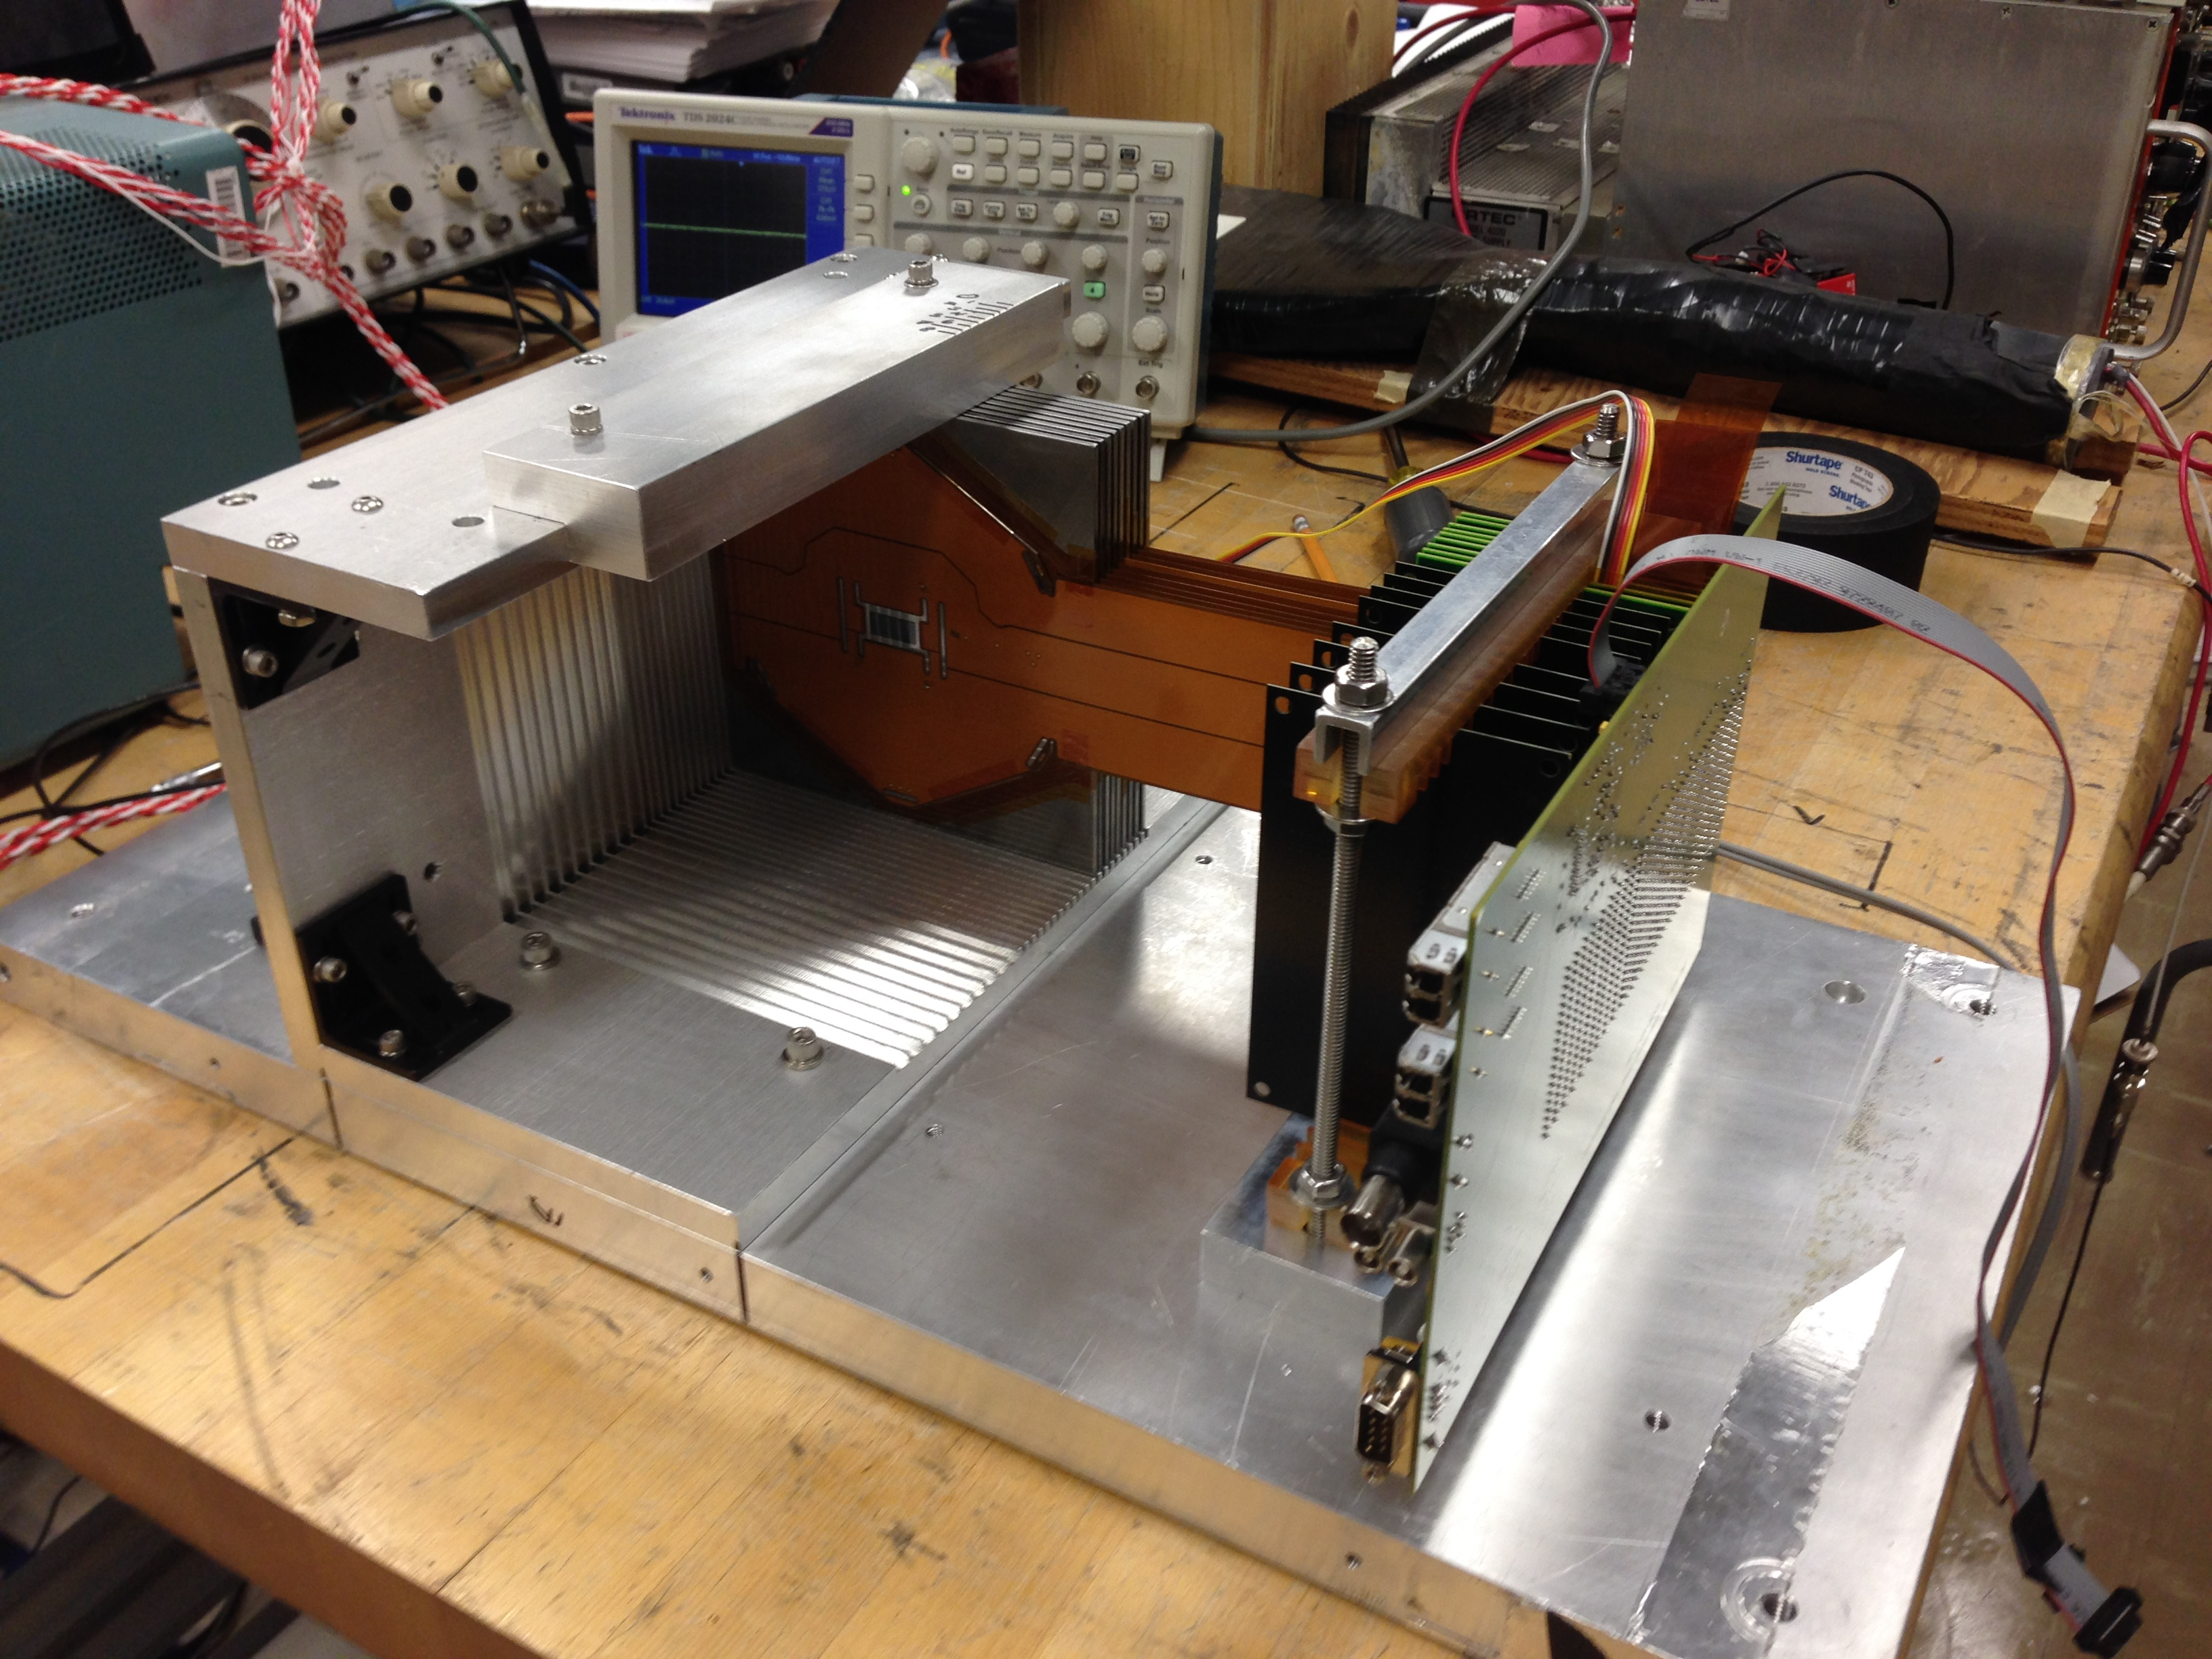
\includegraphics[width=\linewidth,valign=t]{Calorimeter/SiliconTungstenSiD/setup.png}
		\caption{The ECal prototype setup at SLAC, in a silicon-first arrangement.}
		\label{fig:Calorimeter:SiDECAL:setup}
	\end{minipage}
\end{figure}

 In the initial test, a stack of nine silicon sensor planes and eight tungsten plates (corresponding to six radiation lengths) was exposed to beam. Data was taken over a four-day period with a  beam rate between 0.5 and 5 electrons per pulse. The beam was concentrated in a small area of the stack, with mean separation of two electron events of \SIrange{15}{20}{mm}. This data collection provides good measurements of multiple particle overlap and reconstruction of overlapping showers\cite{Steinhebel:2017qze}. Figure~\ref{fig:Calorimeter:SiDECAL:combo} shows the measured total charge distribution for two of the exposure runs compared to a GEANT4 simulation. The distribution was best fit to the simulation assuming a Poisson distribution of beam particles with an average of
0.87. Comparison of the deposited energy distribution in each of the nine layers also agrees well with the simulations.

\begin{figure}
	\centering
	\begin{minipage}[b]{.49\textwidth}
		\includegraphics[width=\linewidth,valign=t]{Calorimeter/SiliconTungstenSiD/combo.png}
		\caption{Prototype runs match very well with GEANT4 simulated data.}
		\label{fig:Calorimeter:SiDECAL:combo}
	\end{minipage}\hfill
	\begin{minipage}[b]{.49\textwidth}
		\includegraphics[width=\linewidth,valign=t]{Calorimeter/SiliconTungstenSiD/tbTagged.png}
		\caption{Distributions of the number of counted electrons.}
		\label{fig:Calorimeter:SiDECAL:tbTagged}
	\end{minipage}
\end{figure}

An algorithm was developed to count the number of incident electrons in each event, based on the total and distribution of energy in each of the nine test beam layers. The algorithm counting was verified with simulated events. Figure~\ref{fig:Calorimeter:SiDECAL:tbTagged} shows the test beam distribution of total energy in the nine layers for each of the counted number of events. The analysis was used to assess the ability of the calorimeter to separate two showers as a function of the separation of the showers. Figure~\ref{fig:Calorimeter:SiDECAL:efficiency} presents the two shower separation efficiency versus separation distance, with 100\% efficiency achieved for $>\SI{10}{mm}$ separation.

\begin{figure}
	\centering
	\begin{minipage}[b]{.49\textwidth}
		\includegraphics[width=\linewidth,valign=t]{Calorimeter/SiliconTungstenSiD/efficiency.png}
		\caption{Efficiency of electron counting algorithm with simulated two electron events.}
		\label{fig:Calorimeter:SiDECAL:efficiency}
	\end{minipage}\hfill
	\begin{minipage}[b]{.49\textwidth}
		\includegraphics[width=\linewidth,valign=t]{Calorimeter/SiliconTungstenSiD/shield.png}
		\caption{Schematic of the shielded sensor.}
		\label{fig:Calorimeter:SiDECAL:shield}
	\end{minipage}
\end{figure}

\subsection{Engineering Challenges}
The first sensors had aluminum pads which required extensive processing to build the Under Bump Metallization (UBM). The sensor foundry now provides the complete UBM, and the bump bonding process (with the KPiX foundry providing the UBM and eutectic solder balls on KPiX) is relatively straightforward.

 Electromagnetic showers can hit a large number of pixels simultaneously. This causes a disturbance in KPiX as many pixels are reset, resulting in a cascade of increasing multiplicity. This problem is understood and requires a small change in KPiX.

 The sensors have traces that cross over other pixels, which is necessary for a small Read Out Chip on the sensor. We have observed crosstalk due to these parasitic couplings, and have designed a new sensor with shielded traces (Figure~\ref{fig:Calorimeter:SiDECAL:shield}). Both the old and new sensors have a metal 1 connection to the diode by a via to metal 2 traces and to the KPiX. In the old version, the metal 1 contact covered the full area of the diode; in the new version, there is only a small connection to the diode, and metal 1 traces run under the metal 2 traces. The metal 1 traces are tied together and held at fixed potential. These sensors have been fabricated and are now being tested.

 Early versions of the sensor cables were bump bonded to the sensor. While this technique uses the least gap height possible, it was too difficult to use efficiently. New cables have been designed that use wire bonded connections, with separate cables for each sensor.

 The forward calorimeters BEAMCAL and LUMICAL have higher occupancy than the barrel and endcaps. It has long been known that the BEAMCAL has an occupancy of about 1, and will use the BEAN\cite{6200898} chip. Studies with Guinea Pig\cite{LCC-0125} pairs only indicate that the LUMICAL may need a readout with more than 4 buffers of KPiX. KPiX will be studied to see if more buffers can be added.

\subsection{Future Plans}
The SiD silicon-tungsten ECal development has been the result of a collaboration of the SLAC National Accelerator Laboratory and the University of Oregon. R\&D has been constrained by a low level of support, so the ECal progress has been limited and slow. Nevertheless, there is now a pre-conceptual mechanical design. The beam test demonstrated expected behavior from the prototype sensors, but also showed significant crosstalk issues in both the sensor and KPiX. There is now a second sensor prototype with trace shielding that is being tested. The KPiX issues are understood, but a new prototype has not yet been built. Evaluation of expected forward multiplicities is ongoing, and may influence the evolution of KPiX.
Final optimization 
of the ECal (layer configuration and number, etc.) will be finished when funding materializes.

%4.4.5   Acknowledgements
%Work supported by the U.S. Department of Energy under contract number DE-AC02-76SF00515 and award number DE-%SC0017996.

\input{Calorimeter/DECAL/DECAL}
\input{Calorimeter/AHCAL/AHCAL}
\input{Calorimeter/SDHCAL_GRPC/SDHCAL_GRPC}
\input{Calorimeter/DHCAL/DHCAL}
\section{THGEM-based sampling elements for DHCAL}
Most recent update: 2020-05-21 \\
Contact person: Shikma Bressler (email: shikma.bressler@cern.ch)
\subsection{Introduction}
Digital Hadronic Calorimetry (DHCAL) for future experiments (e.g. ILC-SiD) requires robust thin sampling elements with high detection efficiency at low pad multiplicity. The large detection area foreseen requires cost-effective solutions.
In recent years, a Weizmann-Aveiro-Coimbra team has shown that sampling elements based on Thick Gaseous Electron Multipliers (THGEM)~\cite{Chechik2004303} could meet DHCAL requirements. The THGEM concept has evolved from a cascade of double-sided electrodes coupled to a pad-anode through an induction gap~\cite{1748-0221-7-05-C05011}, to thinner single-sided WELL detectors - coupled to the pads with and without resistive films~\cite{1748-0221-9-04-P04011,1748-0221-8-07-P07017}.
The most recent and presently leading candidate is the Resistive Plate WELL (RPWELL). It was tested extensively in the laboratory~\cite{1748-0221-8-11-P11004,1748-0221-8-12-C12012} and at muon and high-rate pion beams at CERN-SPS. This very thin single-stage detector yielded a discharge-free operation in different gas mixtures, including Ne- and Ar-based ones, providing high detection efficiency at low pad multiplicity.

\subsubsection{The Resistive Plate WELL}
The Resistive Plate WELL (RPWELL) is a single-sided THGEM (with copper clad on one side only), coupled to the readout pads through a material sheet with high bulk resistivity (see Figure~\ref{fig:Calorimeter:THGEM:rpwell}). Materials with bulk resistivity in the $\SI{e9}{\ohm cm}$ scale prevent significant drops of gain, and hence efficiency, at high particle flux~\cite{1748-0221-8-11-P11004}.
\begin{figure}
	\centering
	\includegraphics[width=.5\textwidth]{Calorimeter/THGEM/rpwell.png}
	\caption{The RPWELL configuration with a resistive anode and a readout electrode. The WELL, a single-faced THGEM, is coupled to a readout anode (e.g. with strips or pads) via a resistive plate.}
	\label{fig:Calorimeter:THGEM:rpwell}
\end{figure}
\subsection{Recent Milestones with Small and Medium Size RPWELL Prototypes}
Small ($10\times \SI{10}{cm^2}$) and medium size ($30\times \SI{30}{cm^2}$) RPWELL detector prototypes were built and tested in the laboratory and at the CERN-SPS. The \SI{0.8}{mm} thick WELL electrodes were coupled to $1\times \SI{1}{cm^2}$ copper pads through \SI{0.4}{mm} thick Semitron ESD225 resistive polymer ($\approx \SI{e9}{\ohm cm}$ bulk resistivity). With a \SI{5}{mm} drift gap the sampling element had a total thickness of \SI{6.2}{mm} (excluding readout electronics -- here SRS-APV~\cite{1748-0221-8-03-C03015,French2001359}).
The detection efficiency as a function of pad multiplicity (with low rate muons) is shown for the two prototypes in Figure~\ref{fig:Calorimeter:THGEM:efficiencyVSMultiplicity}. Both detectors reached high detection efficiency at low pad multiplicity when operated in our traditional Ne/5\%\ce{CH4} (Figure~\ref{fig:Calorimeter:THGEM:efficiencyVSMultiplicity} left; operation voltage, V, in the range $\SIrange{800}{930}{V}$) and in the cost-effective Ar/5\%\ce{CH4} (Figure~\ref{fig:Calorimeter:THGEM:efficiencyVSMultiplicity} right; V in the range $\SIrange{1500}{1720}{V}$) gas mixtures.
\begin{figure}
	\centering
	\includegraphics[width=.9\textwidth]{Calorimeter/THGEM/efficiencyVSMultiplicity.png}
	\caption{Efficiency as a function of the average pad multiplicity measured with the $10\times \SI{10}{cm^2}$ and $30\times \SI{30}{cm^2}$ detectors in muon beam. Left: Ne/5\%\ce{CH4} gas mixture. Right: Ar/5\%\ce{CH4} gas mixture}
	\label{fig:Calorimeter:THGEM:efficiencyVSMultiplicity}
\end{figure}
\begin{figure}
	\centering
	\includegraphics[width=.5\textwidth]{Calorimeter/THGEM/charge_vs_rate.png}
	\caption{The charge (estimated from the spectra most probable value) as a function of the incoming particle flux.  All the measurements were conducted at Ne/5\%\ce{CH4} gas mixture at the same operation voltage of \SI{880}{V}. A pion beam was used to generate the high incoming fluxes.}
	\label{fig:Calorimeter:THGEM:chargeVsRate}
\end{figure}
Figure~\ref{fig:Calorimeter:THGEM:chargeVsRate} shows the measured gain as a function of the particle flux; the same operation voltage of \SI{880}{V} was maintained throughout the measurements (with low rate muons as well as high rate pions). A moderate gain-drop of $\approx 30\%$ was measured while the flux was increased by 3 orders of magnitude (from 50 to $\SI{e5}{Hz/cm^2}$). It resulted in a negligible efficiency drop, since the pulse-over-threshold was sufficiently high.
Most importantly, during the two weeks of in-beam operation (which included also long time operation under high rate, $\SI{e5}{Hz/cm^2}$, pion beam), with both Ne-based and Ar-based gas mixtures, the small prototype was completely discharge-free. The resulting discharge probability is therefore below $10^{-8}$. Occasional discharges occurring in the medium-size prototypes were traced to be associated with defects in some support pins within the active area; these were avoided in the next prototypes.
The RPWELL laboratory and test-beam results with the $\SI{10}\times\SI{10}{cm^2}$ and $\SI{30}\times\SI{30}{cm^2}$ detector prototypes are summarized in \cite{Moleri:2016hgk,Moleri:2016bjv}.

\subsubsection{Preliminary performance of $\SI{50}\times\SI{50}{cm^2}$ RPWELL prototypes}

Having in mind their application to (S)DHCAL, techniques were developed for producing large-area ($\SI{48} \times \SI{48}{cm^2}$) \SI{4.5}{mm} thick (excluding electronics) detectors, incorporating \SI{e10}{\ohm\centi\meter} silicate glass resistive plates (Figure~\ref{fig:Calorimeter:THGEM:glueing}). Five such detectors were built and equipped with a pad-anode embedding ILC-(S)DHCAL MICROROC chips~\cite{Adloff_2012} and has a total thickness of \SI{6.5}{mm}. The RPWELL differed by their electrode quality, of which the thickness variation ranged from 5\% (best) to 25\% (worst), affecting significantly their stability and hence performance.
\begin{figure}
	\centering
	\includegraphics[width=.5\textwidth]{Calorimeter/THGEM/resistivePlateGlueing}
	\caption{The gluing of the glass resistive plate to the pad-anode. Part of the assembly procedure.}
	\label{fig:Calorimeter:THGEM:glueing}
\end{figure}

During August 2018, the first SDHCAL sampling element prototype built (with 25\% thickness variation) has been investigated at CERN/SPS, in Ar/(7\%)CO2, with muons and high-rate pions. Preliminary analysis results confirm that the performance of this prototype would be suitable for (S)DHCAL; $\geq 95\%$ detection efficiency across most of the surface was achieved with a pad multiplicity of $\approx 1$ in most events (average value of 1.7 due to a small number of events with tens of pads firing - probably indicating a discharge). Some efficiency variations are attributed to the large electrode-thickness variations (thus gain). The result obtained with these prototypes as well as those obtained with a small (S)DHCAL comprising several MICROMEGAS, and several RPWELL-based sampling elements are summarized in~\cite{Bressler:2019uyt}.

\subsection{Engineering Challenges}
%The novel design of a large RPWELL detector prototype (without the present support pins) is completed. Assembly and tests are foreseen in the coming year. Upon success, we are confident that future chambers could be fully industrially produced. We are currently investigating, with industry, alternative materials and production technologies of THGEM electrodes; similarly, we are considering different resistive-plate materials, with of appropriate bulk resistivity.

\subsection{Future Plans}
The experience gained with the $\SI{50} \times \SI{50}{cm^2}$ RPWELL prototypes emphasizes the need to use electrodes with much smaller thickness variations, probably below 5\%. It also points towards the need to improve the assembly technique, and in particular ensure that no glue penetrates into the holes. New gluing techniques will be tested in the coming future and the new assembled prototypes will be tested in the laboratory and in muon and pion beams. 
Once suitable sampling elements are built, we foresee additional test beam campaign of an RPWELL or MOGD base (S)DHCAL prototype. 

\input{Calorimeter/GEM_HCAL/GEM_HCAL}
\input{Calorimeter/SDHCal/SDHCAL}
\input{Calorimeter/DualReadout/DualReadout}
\input{Calorimeter/CalorimeterSummary}
\chapter{Forward Calorimeters}
\input{Calorimeter/FCAL/Motivation}
\section{FCAL}
Most recent update: 2020-05-24 \\
Contact person: Wolfgang Lohmann (email: Wolfgang.Lohmann@desy.de)

\subsection{Introduction}
Two special electromagnetic calorimeters are foreseen in the very forward regions of a linear collider detector, denoted hereafter as
LumiCal and BeamCal. In front of BeamCal a layer of pixel detector, denoted as Pair Monitor, will support beam tuning.
\begin{figure}[hbp]
  \centering
   \includegraphics[width=0.45\columnwidth]{Calorimeter/FCAL/figs/forward_region_new} \hfill
   \includegraphics[width=0.45\columnwidth]{Calorimeter/FCAL/figs/BClayer}
  \caption{Left: The very forward region of the ILD detector.
  LumiCal, BeamCal and LHCAL are carried by
  the support tube for the final focusing quadrupole QD0 and the beam-pipe.
  TPC denotes the central track chamber, ECAL the electromagnetic and
  HCAL the hadron calorimeter.
  Right: A half layer of an absorber disk with a sensor sector and front-end electronics.}
  \label{fig:Forward_structure}
\end{figure}
These calorimeters will deliver both a fast and a precise measurement of the luminosity
and extend the detector coverage to low polar angles.
In addition, a LHCal extends the hadron calorimeter coverage to very small polar angles.
Detailed Monte Carlo studies have been performed to
optimize the design of the calorimeters, estimate the background from physics processes and understand the impact
of beam-beam interactions on the luminosity measurement~\cite{2010JInst...512002A}.
A sketch of the design is shown in Figure~\ref{fig:Forward_structure}~(left).

To ensure a high efficiency for single high energy electron detection on top of the large and widely spread
background from beamstrahlung, calorimeters with a small Moli\`{e}re radius are needed. Such compact calorimeters 
also ensure the necessary  precision in the angular reconstruction of Bhabha scattering events.

Due to the high occupancy originating from beamstrahlung and two-photon processes,
both calorimeters need a dedicated fast readout.
In addition, the lower polar angle range of BeamCal is exposed to a large flux
of low energy electrons, resulting in depositions up to one
MGy per year. Hence, radiation hard sensors are necessary.

Compact
cylindrical sandwich
calorimeters using tungsten absorber disks of one radiation length thickness, interspersed with
finely segmented silicon (LumiCal) or GaAs (BeamCal) sensor planes, as sketched in
Figure~\ref{fig:Forward_structure}~(right),
are found
to match the requirements from physics~\cite{2010JInst...512002A}.
LHCal will be designed with a small hadronic interaction length, to fit into the limited space available.

\subsection{Prototype Construction and Beam Tests}

\subsubsection{Currently used Sensors}

Large area GaAs sensors, as shown in Figure~\ref{fig:GaAs} (left), were developed
and produced in collaboration with partners in Russian industry. The Liquid Encapsulated
Czochralski technology is used. The sensors were
doped by a shallow donor (Sn or Te),
and then compensated  with Chromium.
\begin{figure}
\centering
    \includegraphics[width=0.4\columnwidth, height=4cm]{Calorimeter/FCAL/figs/GaAs_sensor_new.jpg}
    \hspace{1cm}
     \includegraphics[width=0.4\columnwidth]{Calorimeter/FCAL/figs/si_proto.jpg}
          \caption{Left: A GaAs pad sensor developed for BeamCal, Right: A silicon pad sensor designed for LumiCal and manufactured by Hamamatsu Photonics.}
    \label{fig:GaAs}
\end{figure}
This results in a semi-insulating GaAs material with a resistivity of about \SI{e7}{\ohm \meter}.
The sensors are \SI{0.5}{mm} thick with pads of a few \si{\milli\meter\squared} area. The operation voltage is about \SI{100}{V} with
leakage current per pad less than \SI{500}{nA}.

Prototypes of LumiCal sensors have been designed
at the Institute of Nuclear Physics PAN
in Cracow~\cite{EUDETMEMO-2009-07} 
and manufactured by Hamamatsu
Photonics.
Their shape, as shown in Figure~\ref{fig:GaAs} (right), is a ring segment of 30\textdegree.
The thickness of the n-type silicon bulk is \SI{0.320}{mm}.
The pitch of the concentric p$^+$ pads is \SI{1.8}{mm} and
the gap between two pads is \SI{0.1}{mm}.
The bias voltage for full depletion ranges between 39 and \SI{45}{V},
and the leakage currents per pad are below \SI{5}{nA}.

\subsubsection{Development of Readout ASICs}

As a first step, dedicated ASICs were designed choosing
an
architecture~\cite{Boie1982365,Gatti:1986qq}
comprising a charge sensitive amplifier and a shaper.
ASICs, containing 8 front-end channels, were designed and fabricated in \SI{0.35}{\micro\meter} CMOS technology.
A variable gain in both the charge amplifier and
the shaper is implemented by a mode switch. The peaking time of the shaper output signal is \SI{60}{ns}.
More results of the measurements of the performance were published elsewhere~\cite{4600902}.
A dedicated low-power, small-area, multichannel ADC is designed and produced~\cite{6156491}.
It comprises eight 10-bit power and frequency (up to \SI{24}{MS/s}) scalable pipeline ADCs and the necessary
auxiliary components.
The readout system containing 32 channels (four pairs of 8-channel front-end and ADC ASICs) was developed and used
successfully in several test-beams, confirming that the chosen readout architecture fulfills the LumiCal requirements.
The main limitation of this ASICs was the number of channels, allowing to build only
small (32 readout channels)  prototype of detector modules. For this reason a new
development of LumiCal readout ASICs called FLAME (FcaL Asic for Multiplane rEadout)
was pursued. The block diagram of FLAME is shown in Figure~\ref{fig:FLAME}. 
\begin{figure}
\centering
    \includegraphics[width=0.9\columnwidth]{Calorimeter/FCAL/figs/FLAME}
    \caption{A block diagram of FLAME readout ASIC.}
    \label{fig:FLAME}
\end{figure}
The FLAME uses the same architecture as the previous readout, with analog front-end and 10-bit ADC in each channel.
The main differences and improvements are listed below. 
\begin{itemize}
\item{FLAME is developed in smaller size TSMC 130~nm CMOS technology.
 This choice allows to obtain large reduction of power consumption and much better radiation hardness}.
\item{FLAME is a System on Chip (SoC) solution comprising all functionality
  (analog front--end, ADC, data serialization and transmission) in one ASIC.
  It will simplify the architecture of the overall readout system and minimise the number of its components.}
\item{FLAME ASICs comprises 32-channels. Designing a readout board with 8 ASICs one can build a detector module
  reading the whole LumiCal sensor tile, containing 256 channels.}
\item{FLAME is built of two identical 16-channel blocks. The data from each block is sent out
  by a very fast (\SI{5.2}{Gbps}) serializer and serial data transmission block. The output data is coded and formatted so that it may be directly received by fast FPGA links.}
\end{itemize}
The development of FLAME has been recently completed. The laboratory tests confirmed that all performance parameters have been matched. Readout boards equipped with FLAME ASICs have been used recently in test-beam measurements of a LumiCal prototype.  

\subsubsection{Data Concentrator and DAQ}

In order to operate a large amount of sensor planes the readout has to be orchestrated.
For this purpose a FPGA based data concentrator is developed.
The prototype of a DAQ module uses a Zynq UltraScale+ FPGA on a Trenz TE0808m board.
The module reads data sent by FLAME, processes and sends them to an external data store using ethernet transmission. 
The current architecture with the generated blocks inside the FPGA is shown in Figure~\ref{fig:FPGA_scheme}. 

\begin{figure}
\centering
    \includegraphics[width=\textwidth]{Calorimeter/FCAL/figs/FPGA_scheme} 
	\caption{Block diagram of the FPGA module used in test-beam measurements.}
    \label{fig:FPGA_scheme}
\end{figure}

\subsubsection{High Quality Tungsten Absorber Plates}

A batch of 25 absorber plates has been fabricated for JINR Dubna by partners in the Russian industry. 
The absorber composition is W 92.5\%, Ni 5.25\%, and Cu 2.25\%.
The material density is \SI{18.0}{\gram\per\centi\meter\cubed}. The thickness of the plates has been assessed using a Zeiss 3D coordinate
measurement system with a precision \SI{2.5}{\micro\meter}. Front and back side measurements were done. The deviation
from planarity is for most of the plates within \SI{50}{\micro\meter} as shown in Figure~\ref{fig:tungsten}.
\begin{figure}
  \centering
   \includegraphics[width=0.9\columnwidth]{Calorimeter/FCAL/figs/tungsten_disk_thickness.jpeg} 
   \caption{Thickness of the tungsten absorber plates. Average thickness and minimum and maximum deviation from planarity is shown.}
  \label{fig:tungsten}
\end{figure}

\subsubsection{Mechanical Stack}

A flexible mechanical structure, as shown in Figure~\ref{fig:mechanical_structure}, has been 
built by CERN as part of the AIDA project,
to compose a technological 
calorimeter prototype instrumented both with LumiCal and BeamCal sensors. 
Tungsten absorber plates, glued on a permaglass
frame, are precisely
positioned on a rod assembly, and interspersed with fully assembled detector planes.
\begin{figure}
    \centering
    \includegraphics[width=0.6\columnwidth,]{Calorimeter/FCAL/figs/mechanical_structure_2}
    \caption{Photograph of the flexible mechanical structure. Tungsten absorber plates, glued on permaglass frames, are put into slots of the
rod assembly.}
    \label{fig:mechanical_structure}
\end{figure}
The flatness of the absorber plates is better than \SI{50}{\micro\meter} to allow for highly compact 
packing of sensor and absorber plates. This stack will be completed 
with absorber plates of the necessary quality up to a total thickness of 30 radiation lengths.

\subsection{Test-beam Measurements}

Test-beams were used to continue radiation hardness studies and study partly instrumented calorimeter prototypes. 
Calorimeter prototypes are built of tungsten absorber plates interspersed with detector  planes as described below. Detector planes comprise a sensor, Kapton fan-outs and FE ASICs.
The first milestones were the measurements in the test-beam of a four
detector plane prototype~\cite{Abramowicz:2017cer} and of a six detector plane prototype~\cite{Abramowicz:2018vwb}. 
Recently, measurements have been performed with a stack instrumented with 11 detector planes, out of which 3 have been operated with the FLAME readout.   

\subsubsection{Radiation Damage Studies}

Two studies of the radiation tolerance of potential BeamCal sensors have
been carried out.
In the first study, the radiation tolerance of prototype GaAs sensors
has been explored by
exposing the sensors to direct radiation from a high-intensity electron
beam of
about \SI{10}{MeV}, which is typical of the energy expected from
beamstrahlung
remnants at ILC. It was found that the sensors can be operated at
room temperature up
to approximately \SI{1}{MGy} without a significant increase in the
leakage current~\cite{1748-0221-7-11-P11022}; however, significant loss
in the response
to ionizing particles was observed. This loss can be partially
compensated, however,
by increasing the bias voltage. In addition, a new round of GaAs:Fe
prototype production
includes a small dopant concentration of iron, which is expected to mitigate
radiation damage effects. Characterization of these new prototypes is
expected soon.

In the second study~\cite{Anderson:2017kkq}, several different
solid-state sensor
technologies were
exposed to varying levels of radiation induced by electrons from the
SLAC End Station A
Test Beam (ESTB).
For this study, the ESTB test beam, with energies varying between 3
and \SI{15}{GeV}, was
directed into a tungsten beam stop. The beam stop was split at the depth
of the shower maximum
and the sensor inserted,
leading to an exposure incorporating the full spectrum of particle
species that will
irradiate the BeamCal sensors. Silicon diode and bulk GaAs, Sapphire and
SiC sensors
were exposed to doses of up to \SI{6}{MGy} of ionizing radiation, along with the
attendant dose of non-ionizing hadronic radiation associated with the
electromagnetic
shower. For GaAs, observed charge collection loss was similar to that of
the first study, although a room-temperature leakage current of
order \SI{10}{\micro\ampere\per\centi\meter\squared}
was observed for \SI{1}{MGy}-scale doses for a sensor
bias of \SI{600}{V}. No significant leakage current was observed for SiC
and Sapphire sensors
irradiated to \SI{0.8}{MGy} and \SI{3}{MGy}, respectively. For these doses, the
charge-collection
loss in SiC was approximately 50\% and for Sapphire, which has low
charge collection
even before irradiation, approximately 75\%. Observed charge
collection loss was
somewhat better for silicon diode sensors: a p-type, float-zone sensor
irradiated
to \SI{6}{MGy} experienced less than 40\% charge-collection loss. However, the silicon
diode sensors developed a significant leakage current. After
beneficial annealing, leakage currents of several hundred \si{\micro\ampere\per\centi\meter\squared}
per MGy of exposure were observed for room-temperature operation at full
depletion
voltage. Lowering the operating temperature to -30\textdegree C reduced
the leakage
current by over two orders of magnitude.
A study~\cite{Schumm:2018phi}
based on a simulation of the BeamCal radiation field
making use of the FLUKA Monte Carlo\cite{Bohlen:2014buj,Ferrari:2005zk}, and damage coefficients
determined from the ESTB results, estimated the accumulated power draw
for a BeamCal instrumented with silicon diode sensors operated
at -30\textdegree C
would be less than \SI{10}{W} per year of operation.

\subsubsection{Performance of a Prototype Calorimeter}

Prototypes of detector planes assembled with FE and ADC ASIC,
as shown in Figure~\ref{fig:fcal_lumical_module_photo},
were built using LumiCal and BeamCal sensors~\cite{1748-0221-7-01-T01004}, and successfully operated in 
test-beam~\cite{Abramowicz:2014gdq}.
\begin{figure}
    \centering
    \includegraphics[width=0.35\columnwidth,angle=90]{Calorimeter/FCAL/figs/tb3_complete_module}
    \caption{Photograph of a fully instrumented detector plane for FCAL.}
    \label{fig:fcal_lumical_module_photo}
\end{figure}
In the next step four detector planes using silicon sensors were used to
study the performance of a prototype calorimeter in an electron and a muon beam. Different numbers of uniform
absorber plates were positioned in front and in between the detector planes in each
run, allowing to study the longitudinal and lateral shower development.
This first prototype, due to the large thickness of the instrumented readout boards, was not as compact as finally needed, but
allowed the demonstration that the multilayer operation and readout is successful. In addition, very good
agreement between data and Monte Carlo simulation
was obtained in the lateral and longitudinal shower development and the precision of the shower position reconstruction. The Moli\`ere 
radius was measured to be \SI{24.0(17)}{mm}.
\begin{figure}
    \includegraphics[width=0.99\columnwidth]{Calorimeter/FCAL/figs/lc_assembly_1.png}
    \caption{Thin LumiCal module assembly. The thickness of adhesive layers (not shown) between components is within \SIrange{10}{15}{\micro\meter}. The total thickness is \SI{650}{\micro\meter}.}
    \label{fig_ThinLCAssembly}
\end{figure}

In following test-beam campaigns eight thin detector planes, as shown in  Figure~\ref{fig_ThinLCAssembly}, 
interspersed by tungsten absorbers of 1 radiation length
thickness were used. The sensors were read out, as an intermediate solution, using 
the APV25 chip~\cite{949881,French2001359} hybrid board. It has 128 channels and two boards read a whole LumiCal sensor. 
Capacitive 
charge dividers were used to enlarge the dynamic range of the APV25 chip.  
The powering circuits and the fan-out part which connects silicon sensor pads with the front-end
board inputs were made from flexible Kapton-copper foils with thickness of \SI{70}{\micro\meter} for the high voltage one,
applied to the back n-side of the sensor and about \SI{120}{\micro\meter} for the fan-out.
Ultrasonic wire bonding was used to connect conductive traces on the fan-out to the sensor pads.
A support structure made of carbon fiber composite with a thickness of \SI{100}{\micro\meter} in the sensor-gluing area
provides mechanical stability. 
The ultrasonic wire bonding proved to provide good electrical performance, but for a detector plane thinner than \SI{1}{mm}, the wire loops,
which are typically \SIrange{100}{200}{\micro\meter} high, cause a serious problem when the module needs to be installed in a \SI{1}{mm} gap between absorber plates.
The bonding machine was tuned to make the loop as low as possible and technically acceptable.
The sampling based measurements, which were done using a con-focal laser scanning microscope, show that the loop
height is in the range \SIrange{50}{100}{\micro\meter}. The total thickness of the detector plane was \SI{650}{\micro\meter}.

The calorimeter prototype was studied in a \SIrange{1}{5}{GeV} electron beam at DESY~\cite{Ghenescu:2018sow,Abramowicz:2018vwb}. The shower position was reconstructed with a resolution of \SI{440(20)}{\micro\meter}.
The average transverse shower profile is shown in 
Figure~\ref{MR_5GeV} for data and Monte Carlo simulation. Very good agreement is found. The effective Moli\`ere radius is
determined to be \SI{8.1(3)}{mm} in data and \SI{8.4(1)}{mm} in Monte Carlo simulations.

\begin{figure}
    \centering
    \includegraphics[width=\textwidth]{Calorimeter/FCAL/figs/MR_5GeV_EffS_v3.pdf}
    \caption{The average transverse shower profile, $\langle E^{det}_{n} \rangle$, as a function 
of the distance from the core, $d_{core}$, in units of pads, for data (blue triangles) and MC 
simulation (red circles). The histograms are the results of fits to data and MC using a parametrisation of the 
shower shape. The lower part of the figure shows the ratio 
of the distributions to the fitted function, for the data (blue) and the MC (red).}
    \label{MR_5GeV}
\end{figure}
In a recent test-beam campaign part of the calorimeter prototype was equipped with FLAME read-out boards and an FPGA data concentrator. Several millions events have been recorded in the same electron beam mentioned above. The data analysis is still ongoing.

\subsection{Engineering Challenges}
Engineering challenges within the current and future research of FCAL are the following:
\begin{itemize}
\item A slim assembled detector plane. First prototypes of a ultra-thin detector planes have been successfully
manufactured and used in test-beam measurements.
These technologies need to be completed and transferred into mass production. 
\item Miniaturized PCBs using FLAME chips, to be applicable in an experiment 
\item Development of readout ASICs for BeamCal.
Here prototypes are designed, and a submission is planned soon.
\item Operation using power pulsing to avoid active cooling.
\item A dedicated solution for data concentration, data reduction and transmission, allowing read out of 
the full calorimeters after each bunch crossing.
\item Precise alignment and position monitoring. The inner radius of LumiCal has to be controlled with a precision
of about \SI{10}{\micro\meter}, and the distance between the 
calorimeters on both sides of the IP with a precision of \SI{100}{\micro\meter}.
\item Montage and demontage of the calorimeters must be done when the beam-pipe is installed. The calorimeters must be segmented at 
least in two half cylinders, and corresponding auxiliary mechanics has to be developed.
\end{itemize}

\subsection{Future Plans}

\subsubsection{Novel Sensor Materials}

The performance of single crystal Sapphire sensors to detect minimum ionising particles has been studied for the 
first time~\cite{1748-0221-10-08-P08008}. Sapphire sensors are a promising alternative for GaAs to instrument
the region near the beam-pipe where a high radiation field is expected.

With Hamamatsu Photonics the design of 
edge-less silicon sensors is under preparation. Using edge-less sensors in LumiCal would avoid performance losses 
in gaps between sensor segments.

\subsubsection{Technological Calorimeter Prototype}

Currently the goal of FCAL is to prepare a full depth calorimeter prototype instrumented with more than 20
detector planes equipped with FLAME read-out for test-beam measurements. These measurements
are essential firstly to develop and test engineering solutions to build a very compact calorimeter and
secondly to verify the results of Monte Carlo studies. Depending on the test beam
results the calorimeter may be redesigned.
For the prototype calorimeter
a mechanical structure, a sufficient amount of ASICs, FPGAs for
data concentration and
a data acquisition system are needed. In addition, 
two-planes of a pixel tracker in front of LumiCal will be prepared to improve the polar angle resolution.

\subsubsection{Alignment and Position Monitoring }

A laboratory set-up for position monitoring has been constructed by IFJPAN Cracow using semi-transparent
silicon sensors~\cite{EUDETREPORT-2008-05}. Test measurements demonstrated that position monitoring 
with \si{\micro\meter} precision is possible. A design how to integrate the system in a larger detector has still to be developed. 

\subsubsection{Front-End and ADC ASICs}

Engineering solutions for a miniaturized FLAME readout boards will be developed, and an amount of ASICs will be fabricated
to be used in the larger calorimeter prototype.

A dedicated ASIC development is ongoing for BeamCal~\cite{6200898}
with a special option for a fast readout of a reduced amount of
information from a few bunch-crossings to be used for a fast feedback system for beam-tuning~\cite{1748-0221-3-10-P10004}.
A small prototype of a pixel sensor readout for the pair monitor, positioned in front of BeamCal was designed in SoI
technology~\cite{Sato201153}. This development is foreseen to be continued.

\subsubsection{Data Acquisition}

Ongoing further work will focus on the ethernet transmission.The higher level DAQ will depend on the functionality of the 
data concentrator. For the readout of test-beam data software is developed, mainly by the University of Tel Aviv,
which can be easily adopted. For the final device FCAL will follow the developments of a common DAQ for all detectors.

\input{Calorimeter/FCALSummary}
\chapter{Muon Detector}
\input{MuonDetector/Motivation}
\input{MuonDetector/MuonDetectorILD/MuonDetectorILD}
\input{MuonDetector/Scintillator/Scintillator}
\input{MuonDetector/MuonSummary}
\chapter{Software Tools}
Most recent update: 2016-04-29\\
Contact person: Frank Gaede (email: frank.gaede@desy.de)
\input{Software/Introduction}
\input{Software/LCIO/LCIO}
\input{Software/DD4HEP/DD4HEP}
\input{Software/Marlin/Marlin}
\input{Software/PandoraPFA/PandoraPFA}
\input{Software/LCFIPlus/LCFIPlus}
\input{Software/SoftwareSummary}
% \input{Software/Executive_Summary}
\chapter{Spinoffs}
\input{Spinoffs/Spinoffs}
\printbibliography
\end{document}
